\documentclass{DeustoFDP}
\usepackage{hologo} % Paquete no necesario. Borrar en la memoria final al sustituir el texto
\hypersetup{
pdfauthor={Aitor Brazaola Vicario},
pdftitle={Final Degree Project - Aitor Brazaola. University of Deusto},
}

\bibliography{bib}

\begin{document}

\frontmatter
\pagestyle{plain}

% Las siguientes lineas (21--26) se pueden eliminar del documento final.
% Notese que en ese caso es necesario descomentar la linea 28 para que las
% paginas esten correctamente numeradas.
\begin{titlepage}
    \newgeometry{left=0cm,right=0cm,bottom=0cm,top=0cm}
    
\includegraphics{fig/portada}
    \restoregeometry
\end{titlepage}
\cleardoublepage

\setcounter{page}{3}

\chapter*{Abstract}
The lifestyle of today's society moves away the traditional contact between neighbors
where is promoted the goods, services and information exchange between citizens. In addition, the growth of cities makes more difficult for councils and public institutions being aware of needs and concerns of the inhabitants.

Auzonet as digital platform focused on the residents, provides the perfect solution to neighbors providing a web platform to exchange relevant information and being a reliable data source for public institutions.

\vspace{2em}

{\Large\bfseries\sectionfont Keywords}
\vspace{3\medskipamount}

OpenData, Web, App, Social network.

\cleardoublepage\tableofcontents
\cleardoublepage\listoffigures
\cleardoublepage\listoftables
\cleardoublepage\listoflistings

\mainmatter
\pagestyle{phdthesis}

\chapter{Introduction}\label{cha:introduction}
The aim of this project is create an online social platform for benefit different parties, on the one hand, the Bilbao's council citizens, building a meeting point in the community for posting warnings or relevant information with other people living in the same neighborhood, and publishing requests or offers to help among them.

On the other hand, the information generated by the platform usage can be a source of high-quality data for council's services improvement, allowing these institutions to take better decisions for improve the life quality of the city.

This project must be developed using resources of European project WeLive~\cite{WeLive} which DeustoTech~\cite{DeustoTech} MORElab~\cite{Morelab} belongs to, using their libraries and programming interfaces for obtaining Bilbao's council Open Data. 

WeLive is a web platform to promote OpenData in institutions created by several European entities that provides a range of services for developers and public entities to facilitate Open Data usage in third-party applications.

The main challenges will tackle this project are:

\begin{itemize}
    \item Create a social web platform easy to use to promote users collaboration.
    \item Add value to the platform using public datasets.
    \item Learn to develop a full-stack web and mobile application.
\end{itemize}

In addition, during the development may be necessary develop new reusable software components for allow WeLive custom integrations and make it available in the application repository of WeLive platform.

This project will need technical and interpersonal skills to achieve good collaboration between WeLive and Auzonet teams to build the best quality software.

To carry out major development of the project, will be used a web framework for building the web application with maximum code reuse and better efficiency, for developing mobile application, a portable version of the web will be embedded using multi-platform deployment tools.

The previously mentioned tools add the challenge of make a web design responsive for adapt all visual components to different smartphone's screen sizes  and learn how to communicate applications via API's that requires WeLive to interact with public data.

All phases of development will put in manifest the knowledge acquired during the university degree and require new technical and theoretical skills.

This document describes the project, how has be planned, developed, the objectives and procedures to make good usage of public data released by institutions adding value to services offered by cities to citizens.

In the development chapter internal process will de explained in detail, reasoning the tools finally used and the why has been chosen, the project structure and possible functional divisions of software components, design and requirements.


Finally, the last chapter include conclusions found throughout the entire process of creation and improvements to the platform for future updates.

\chapter{Background and rationale}\label{cha:backgroundandrationale}
\section{Background}
The aim of this project is create a social network for neighbors, using public data for avoiding error during users registration and making good usage of public datasets, but as can be seen in the following state of art study, this is not the first initiative taken in this field.
\subsection{Social network for neighborhoods}
Creating a social network for neighbors in which all members of a portal or community can interact with each other by sharing resources and information is not a new initiative, in other countries like Germany or United States similar projects \cite{larazon} have been developed, internet has extended the creation of communities of all kinds of areas, however, the already existing proposals rarely get benefit of the public entities data, and in many cases, they are the most reliable source of information for building applications and services for citizens.

\begin{figure}[H]
\centering
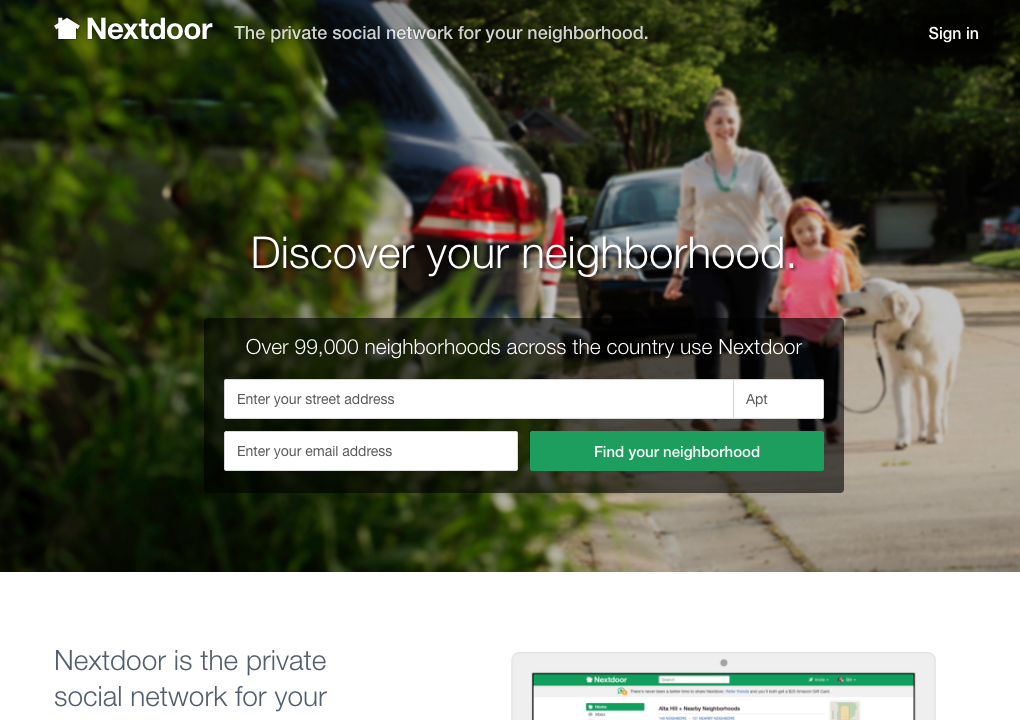
\includegraphics[width=0.7\linewidth]{fig/nextdoor}
\caption[Nextdoor]{Nextdoor. Existing alternative in USA.}
\label{fig:nextdoor}
\end{figure}


\subsection{Open Data}
Although it is true that currently, many public entities make available this data in digital format only by the look of transparency and are unaware of the true value of themselves, is one of the motivation of this project, in fact, have been moments during the development in which the data found poorly formatted and have had to request modifications to the agencies involved.

The fact that most of datasets that are published by public organizations are not used in systems created by third parties, causes certain unconcern in the status and integrity of them.

\section{Rationale}
This project aims to unify the capabilities of communication between people that internet provides with the benefits of the Open Data to citizens, something that rarely have been done in similar intiatives.

\chapter{Goals and scope}\label{cha:goalsandscope}
\section{Project definition}
Auzonet must meet the expectations of at least two types of users:
\begin{description}
	\item[Citizen:] It is the primary user of the system and the beneficiary of the features offered by the platform and the source of the information that the system creates for later exploitation.
	\item[Public institution:] It who analyze the data generated by the platform for statistics and promoting services that improve the quality of life in cities and people.
\end{description}

To achieve this it will develop:
\begin{itemize}
	\item A web application where users can register their neighborhood based on existing data published by the council of Bilbao, the rest of neighbors interested can join to it and get benefit from its functions.
	
	\item A mobile application that lets you interact with the main functions of the web from a smartphone.
\end{itemize}

\subsection{Functionality}
Users can search their portal trough an interactive form based on the existing neighbors and streets of the city of Bilbao, for better confirmation of the place, a small map showing the exact situation of the door will be displayed, if the information is correct, a few setting should be configure like the privacy level of the community having the option to protect it with a password or add a few lines of welcome message to new members via mail.

Each user can belong to more than one community of neighbors, considering that may want to be aware of the community of their usual residence and for example the holidays.

Each neighborhood community represented in the application has its own home page where you can see the cork with warnings or information notes published and a lower table divided into two sections called Requests and Offers where will be displayed the posts created by members of that community.

From the home page of each community, the user can create a request for a product or service or to publish an offer in which can specify whether you want to get paid or offer the service for free.

To ensure some confidence when working with another user, a karma level system represented by a numeric value that is higher or lower by other users past reviews determine the trust level of each user.

\subsection{Limitations}
Auzonet never going to manage payments among individuals, beyond the simple fact of a history of interactions between requests and offers between neighbors. Interested parties should agree on a transaction which methods used to pay if they require and have the complete responsibility for ensuring the successful transaction in a legal economic frame.

Will be the users themselves who in case to use the platform will have to register their portal in the section for creating communities to make use of the software functions.

There are no plans to develop applications with the native development kit of each mobile operating system for avoiding multiple processes of simultaneous development during the creation of the mobile application, web technologies to deploy the application available on the market will be used.

\section{Description of the embodiment}
\subsection{Development methodology}
The realization of Auzonet is separated in two main functional units, first will focus on finalizing the web application and then mobile app.

As can be seen in the figure \ref{fig:edt} the development phases are going to be the following:
\begin{description}
	\item[Requirements:] Analysis of the main functional requirements.
	\item[Design:] Design data and logical structures needed for running the application and approach to the aesthetic design of the solution.
	\item[Web application development:] Implementation process of the main application, with Welive project integration and "responsive" design for fitting on different screen sizes.
	\item[Mobile application development:] Implementation process of mobile application that get benefits of the "responsive" design of the web application.
	\item[Tests:] Different executions by end users and bug detection on the feature usage processes for debugging, It will try to involve collaborators and friends of the programmer for making real usage of the platform.
\end{description}

Being a project that involves only one developer will not be used agile methodologies that facilitate cooperation and teamwork, instead, a system of lists of tickets with different classifications will be used in a task manager software.

Tasks are classified as follows:
\begin{table}[H]
	\centering
	\caption{Ticket categories.}\label{tab:ticketcategories}
	\begin{tabular}{cccc}
		\toprule
		\textbf{Category} & \emph{Description}\\
		\midrule
		Functional  & Features that represent the core of the application.\\
		Not functional   & Features that enrich the user experience.\\
		Bug & Faults to debug.\\
		Improvement & Suggestions or new functionalities that add value to the platform.\\
		\bottomrule
	\end{tabular}
\end{table}

Sometimes, certain tasks can come from external sources such as suggestions for improvement or major deficiencies found in a test, in that case, they are added to the list with the corresponding label and prioritized according to their importance.
\subsection{Intermediate products}
\begin{itemize}
	\item Web application.
	\item Public data integrated via WeLive platform.
	\item Mobile application.
\end{itemize}
\newpage
\begin{figure}[H]
	\centering
	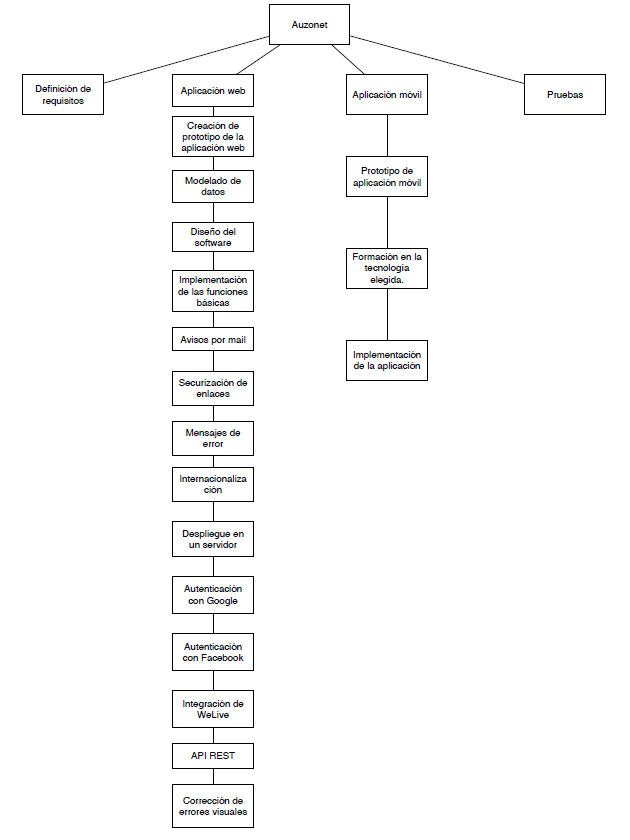
\includegraphics{fig/EDT}
	\caption{EDT}\label{fig:edt}
\end{figure}
\subsection{Main tasks}
\begin{figure}[H]
	\centering
	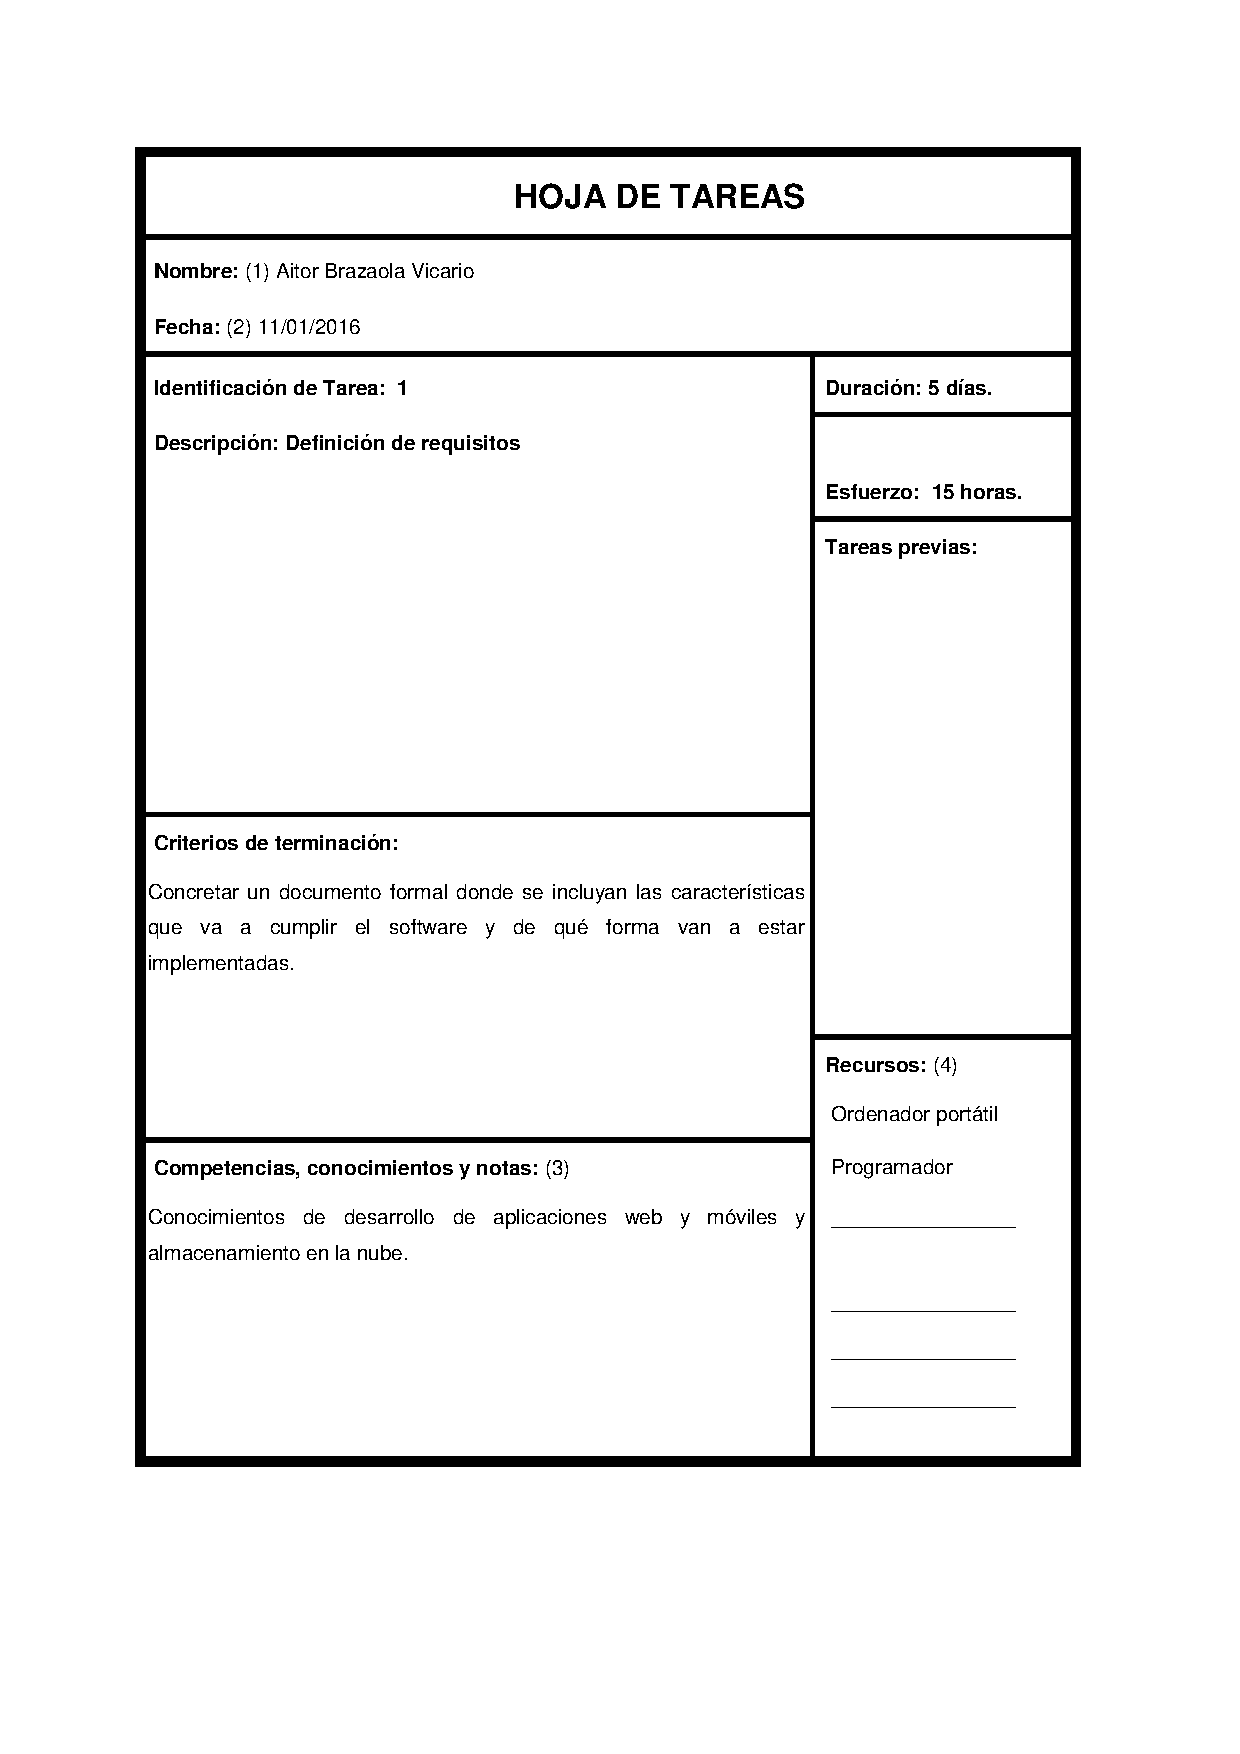
\includegraphics[width=0.9\textwidth]{fig/Tareas/1}
	\caption{Task 1}
	\label{fig:t1}
\end{figure}

\begin{figure}[H]
	\centering
	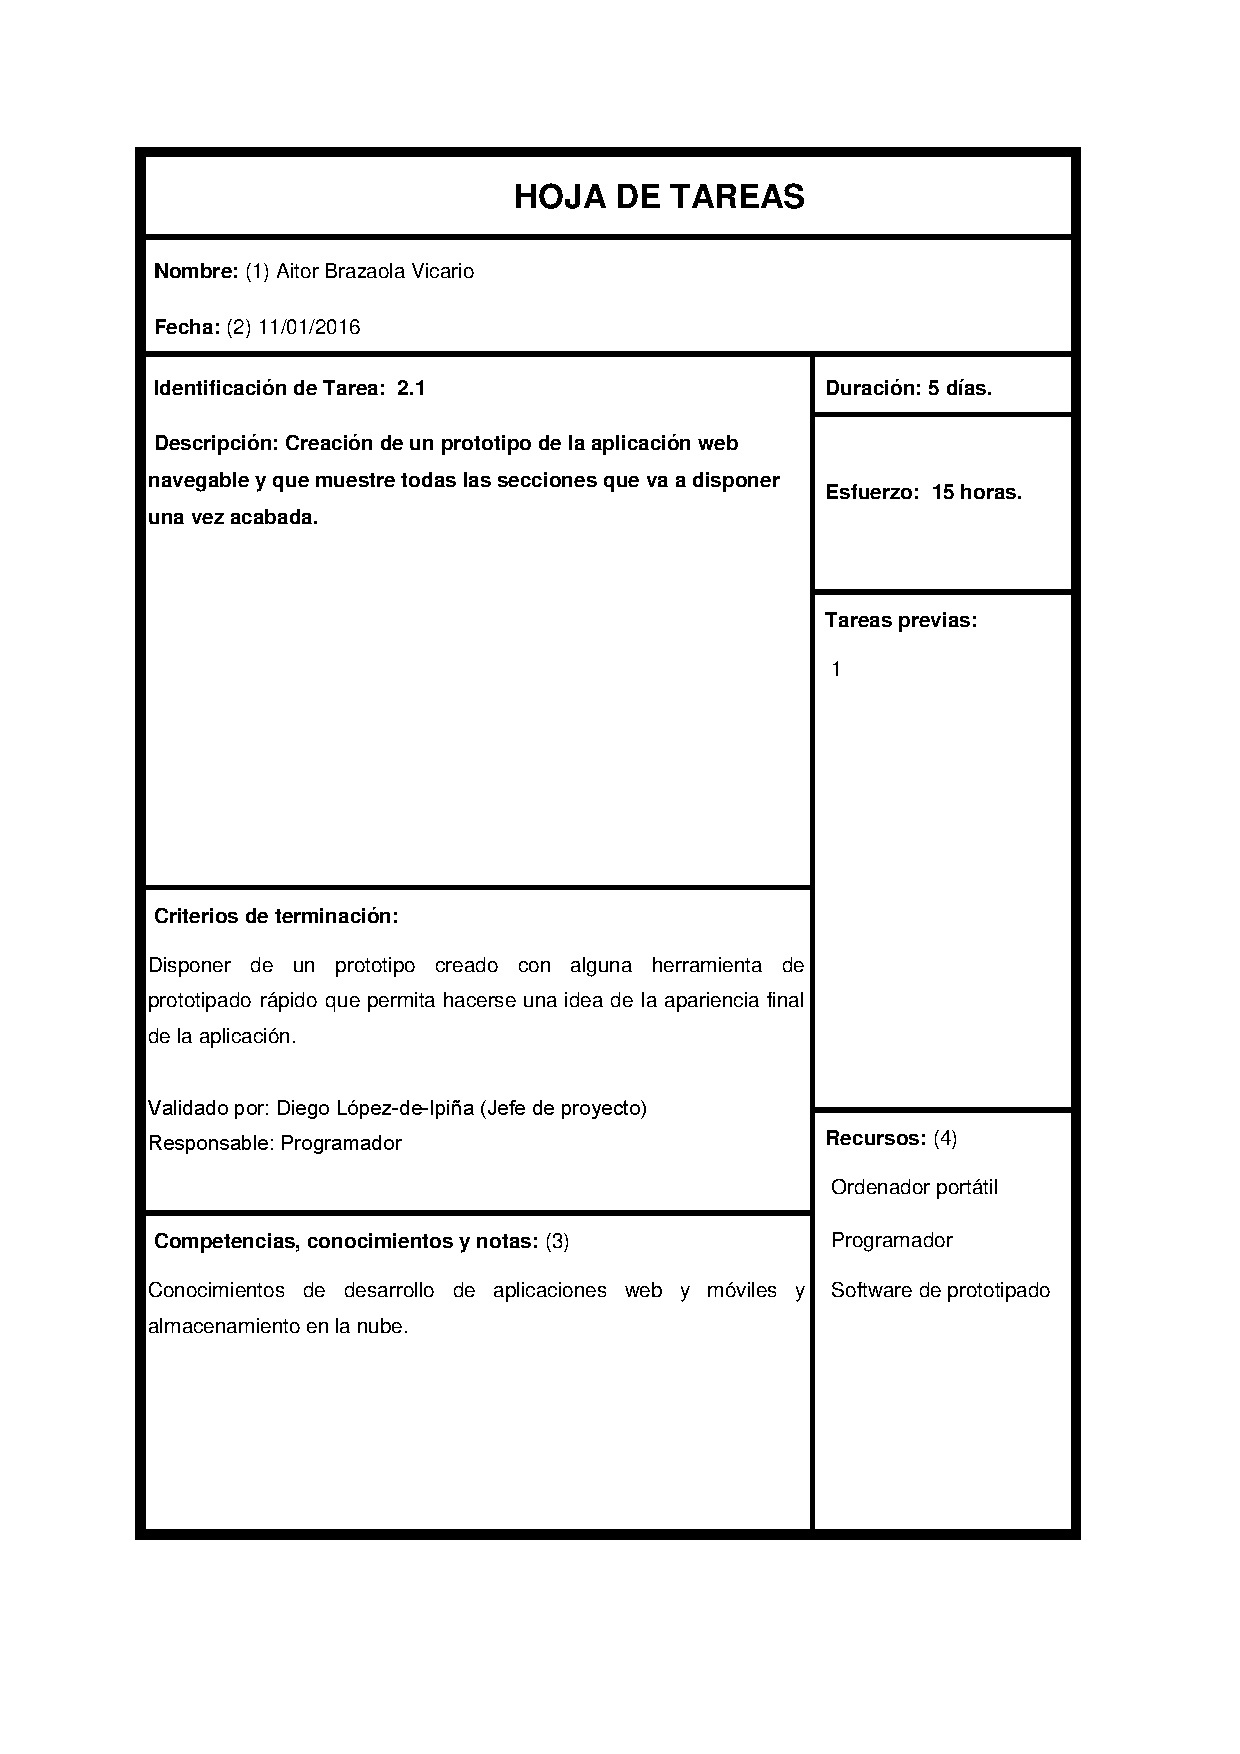
\includegraphics[width=0.9\textwidth]{fig/Tareas/21}
	\caption{Task 2.1.}
	\label{fig:t21}
\end{figure}

\begin{figure}[H]
	\centering
	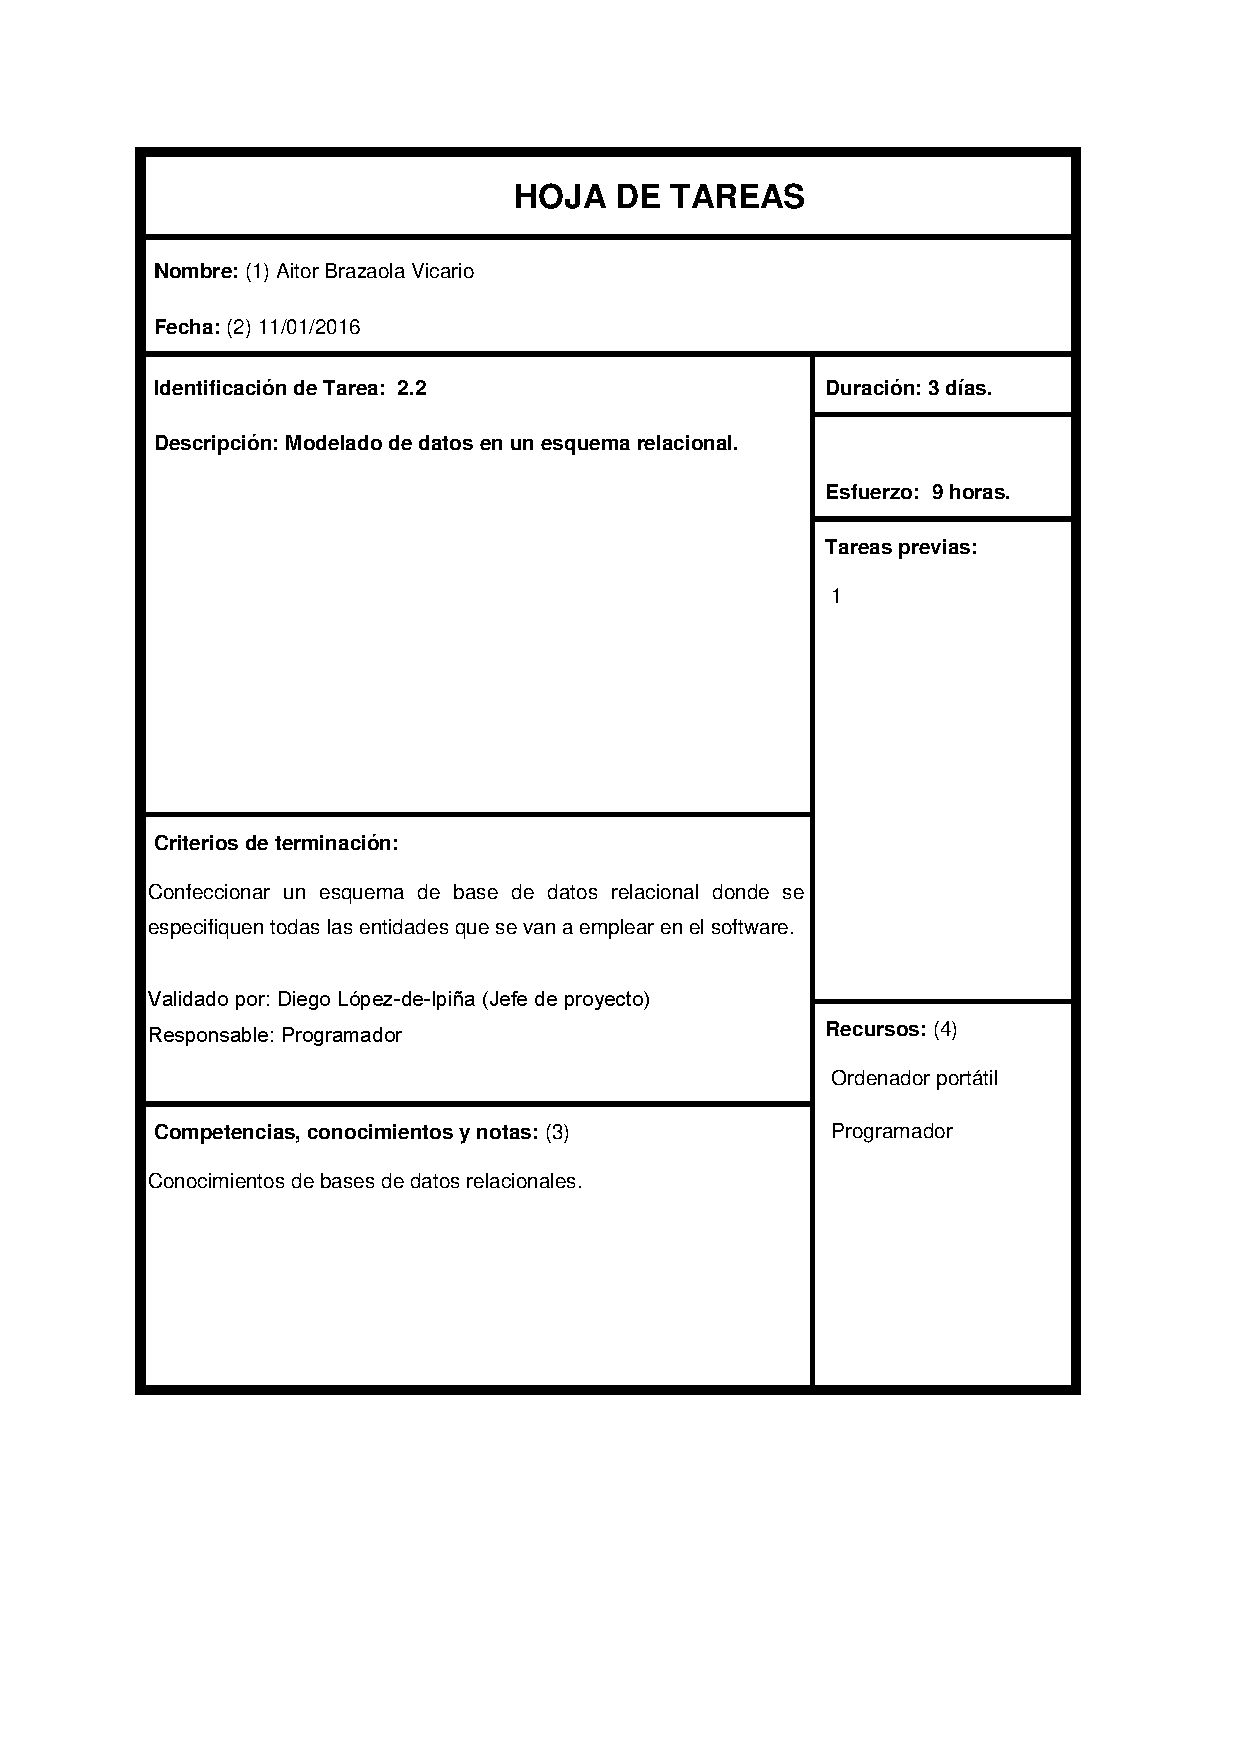
\includegraphics[width=0.9\textwidth]{fig/Tareas/22}
	\caption{Task 2.2.}
	\label{fig:t22}
\end{figure}

\begin{figure}[H]
	\centering
	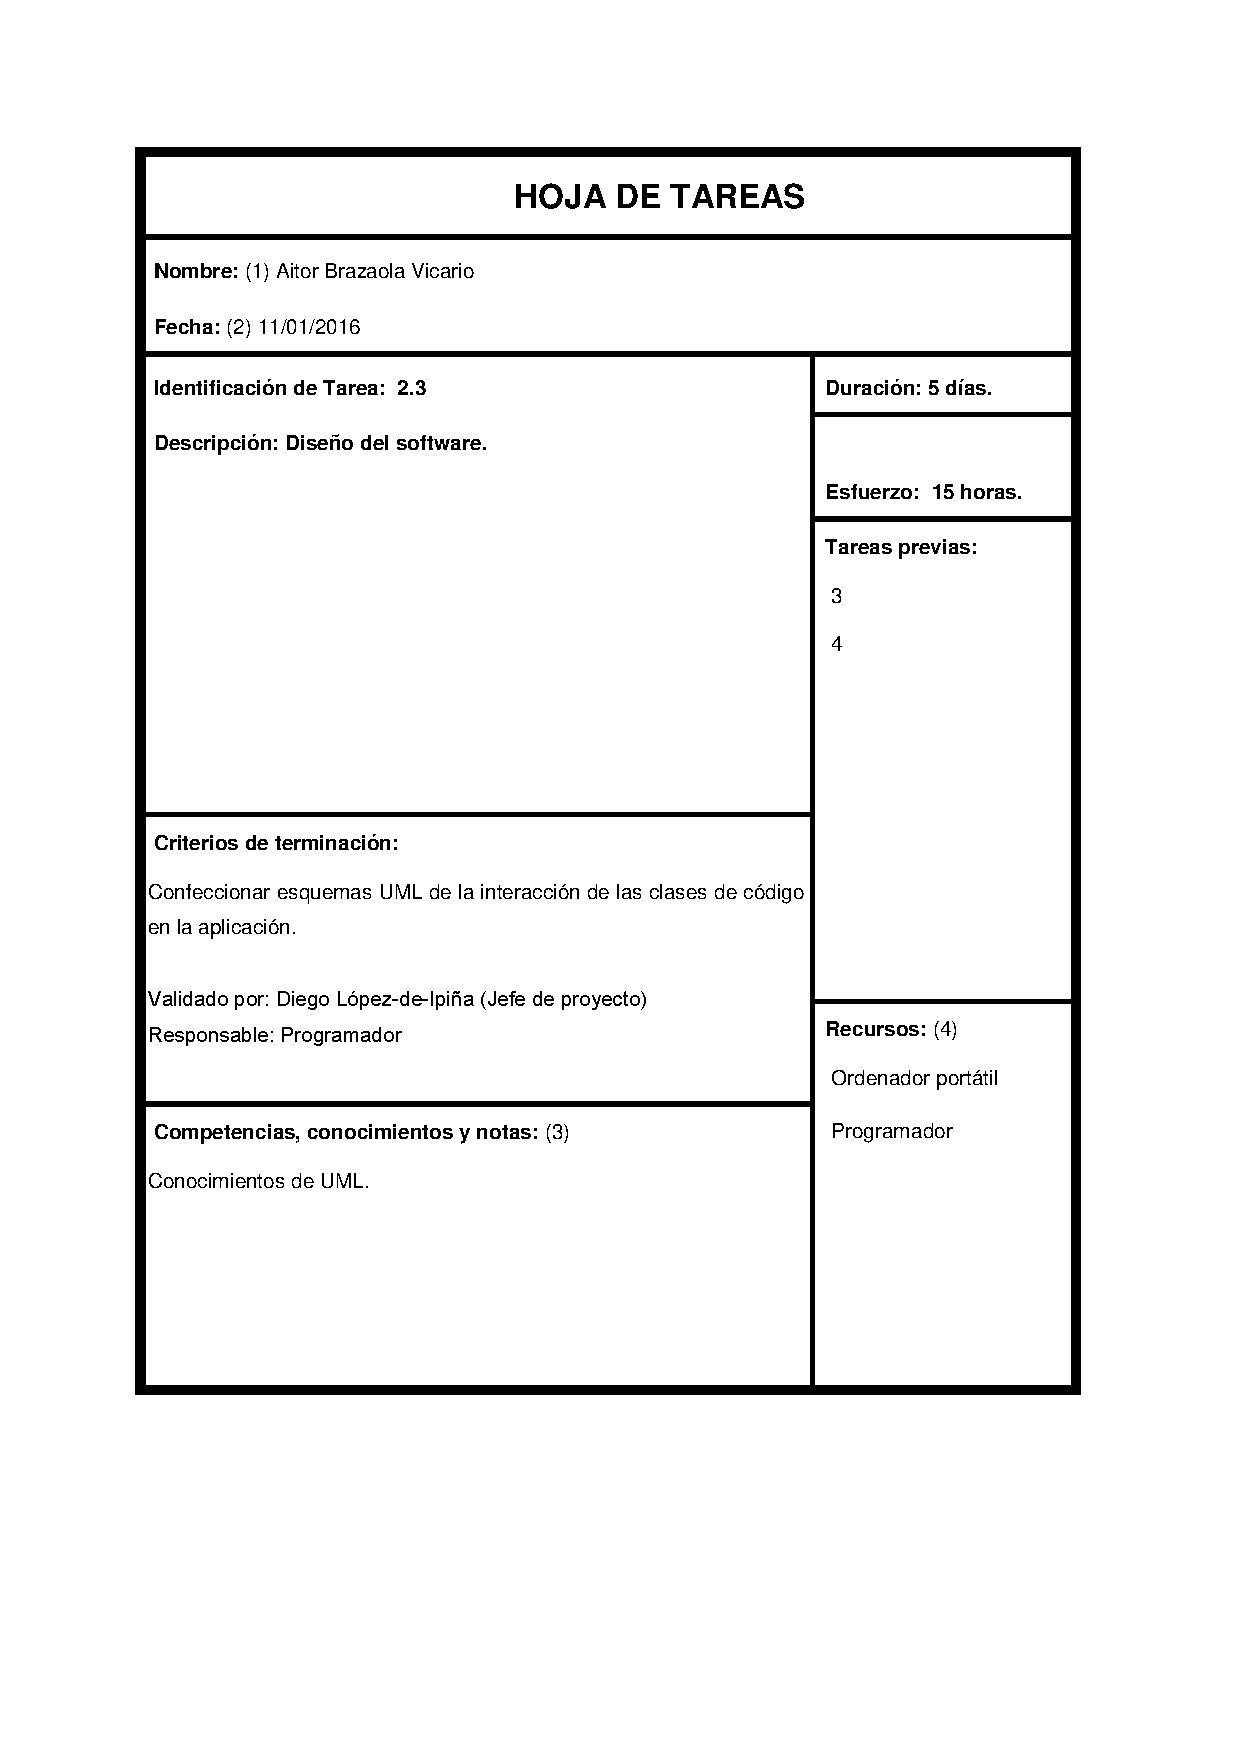
\includegraphics[width=0.9\textwidth]{fig/Tareas/23}
	\caption{Task 2.3.}
	\label{fig:t23}
\end{figure}

\begin{figure}[H]
	\centering
	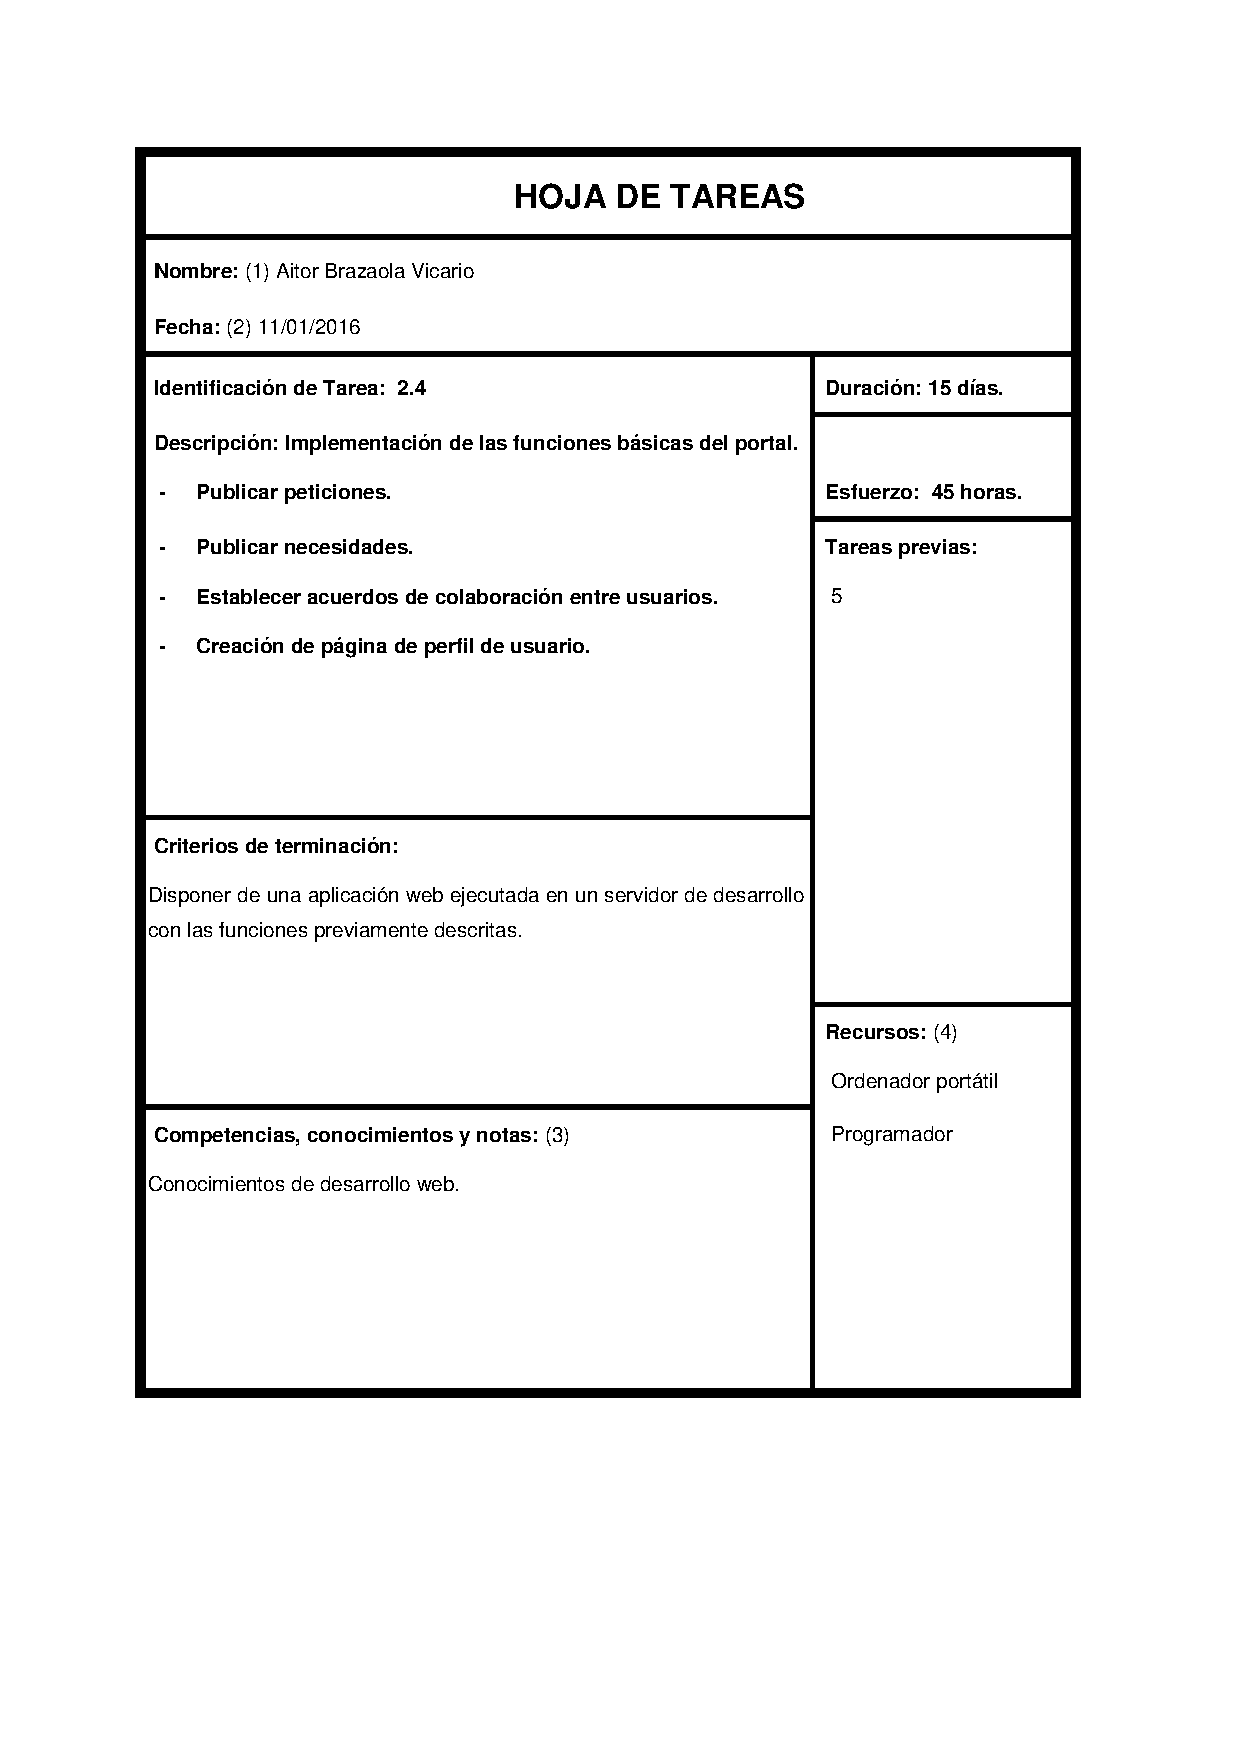
\includegraphics[width=0.9\textwidth]{fig/Tareas/24}
	\caption{Task 2.4.}
	\label{fig:t24}
\end{figure}

\begin{figure}[H]
	\centering
	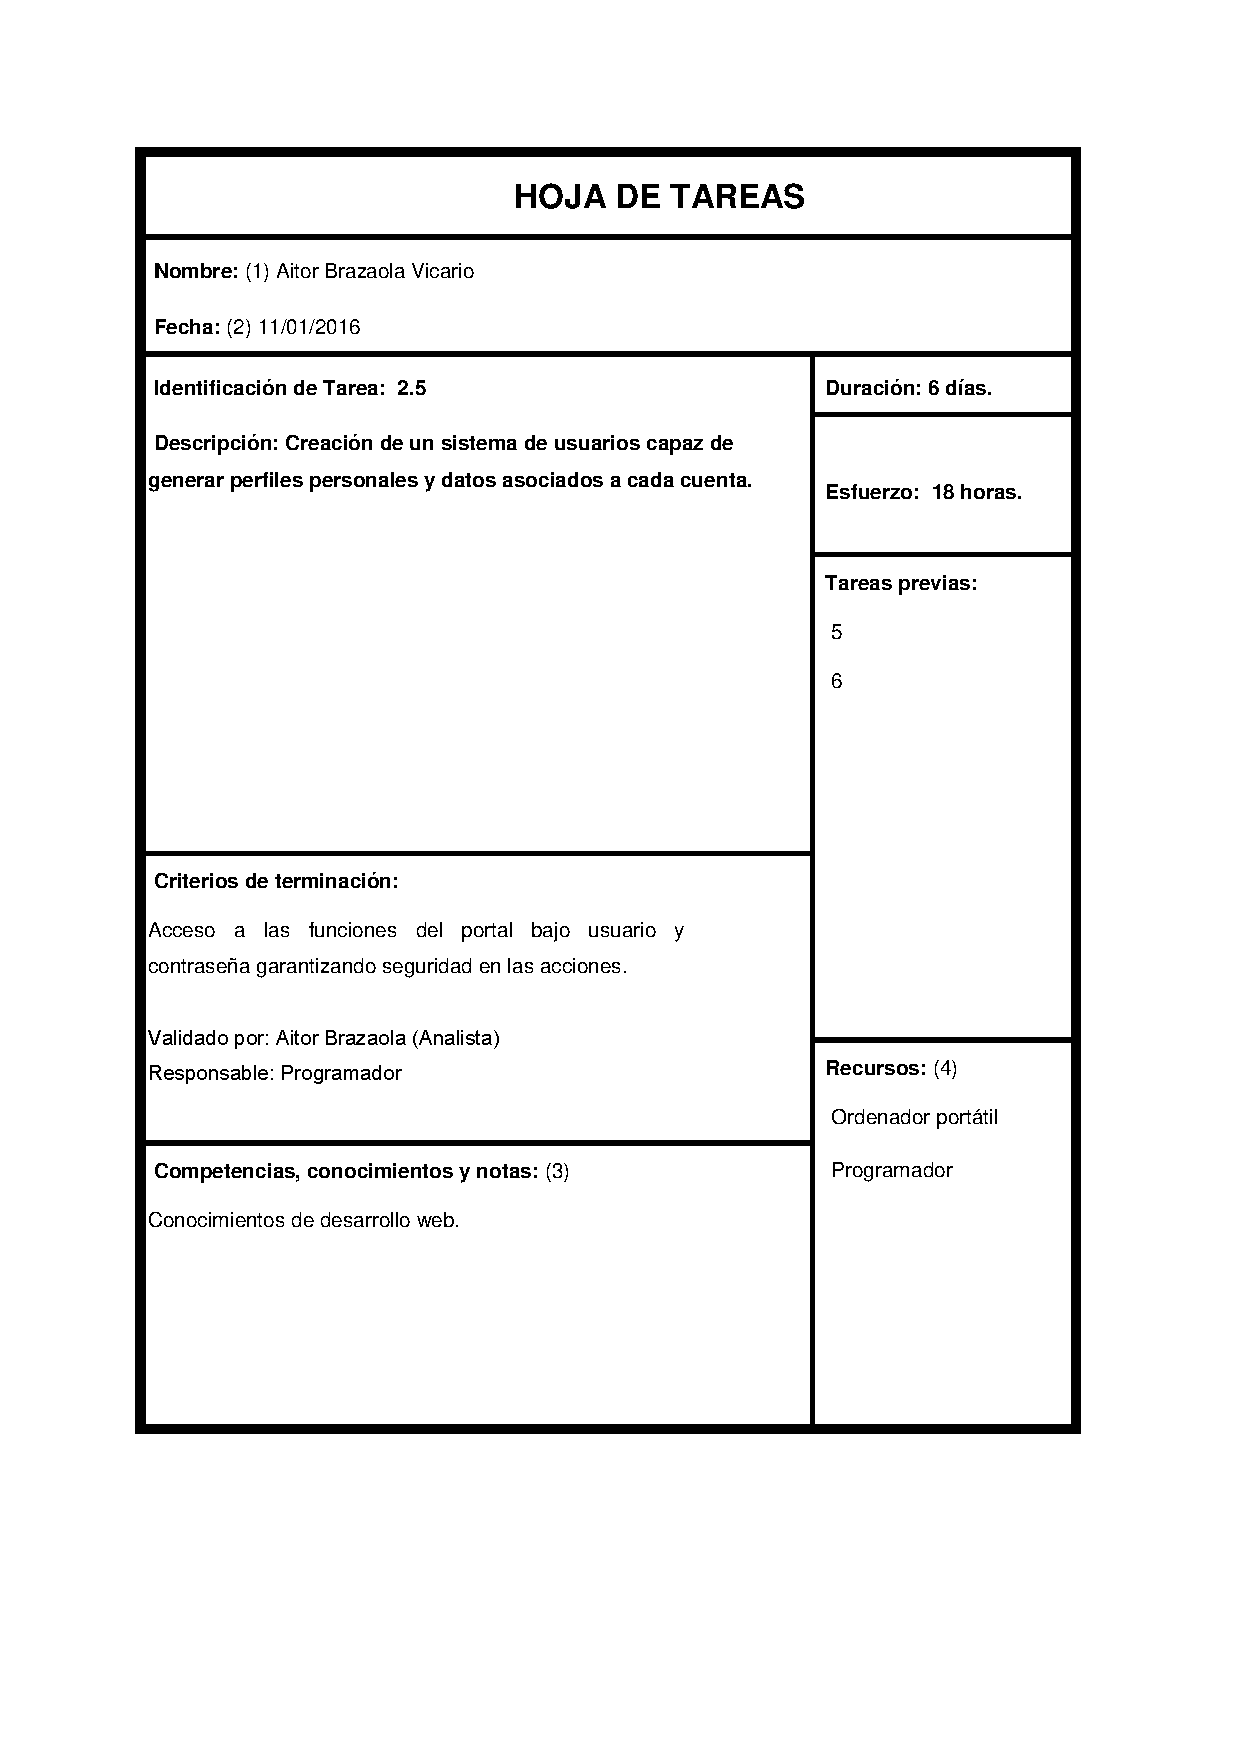
\includegraphics[width=0.9\textwidth]{fig/Tareas/25}
	\caption{Task 2.5.}
	\label{fig:t25}
\end{figure}

\begin{figure}[H]
	\centering
	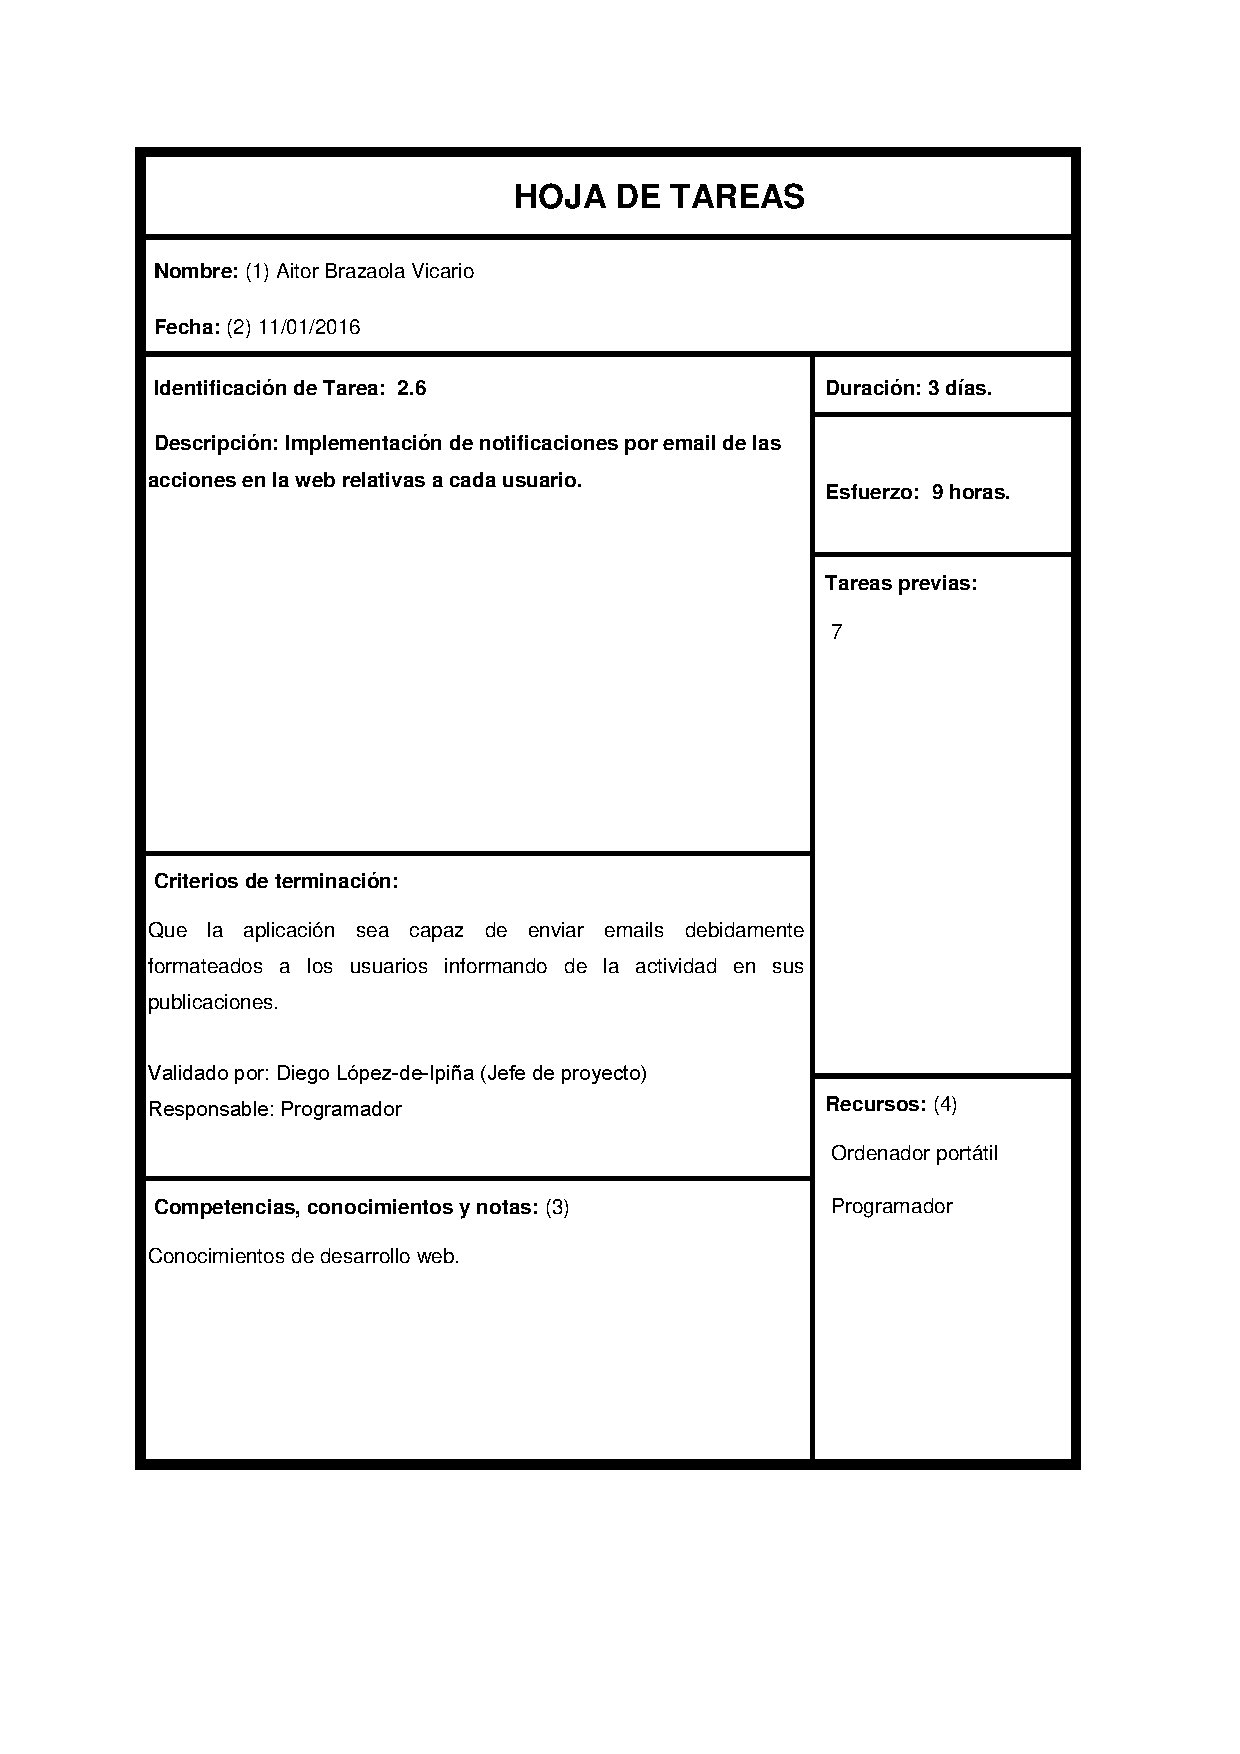
\includegraphics[width=0.9\textwidth]{fig/Tareas/26}
	\caption{Task 2.6.}
	\label{fig:t26}
\end{figure}

\begin{figure}[H]
	\centering
	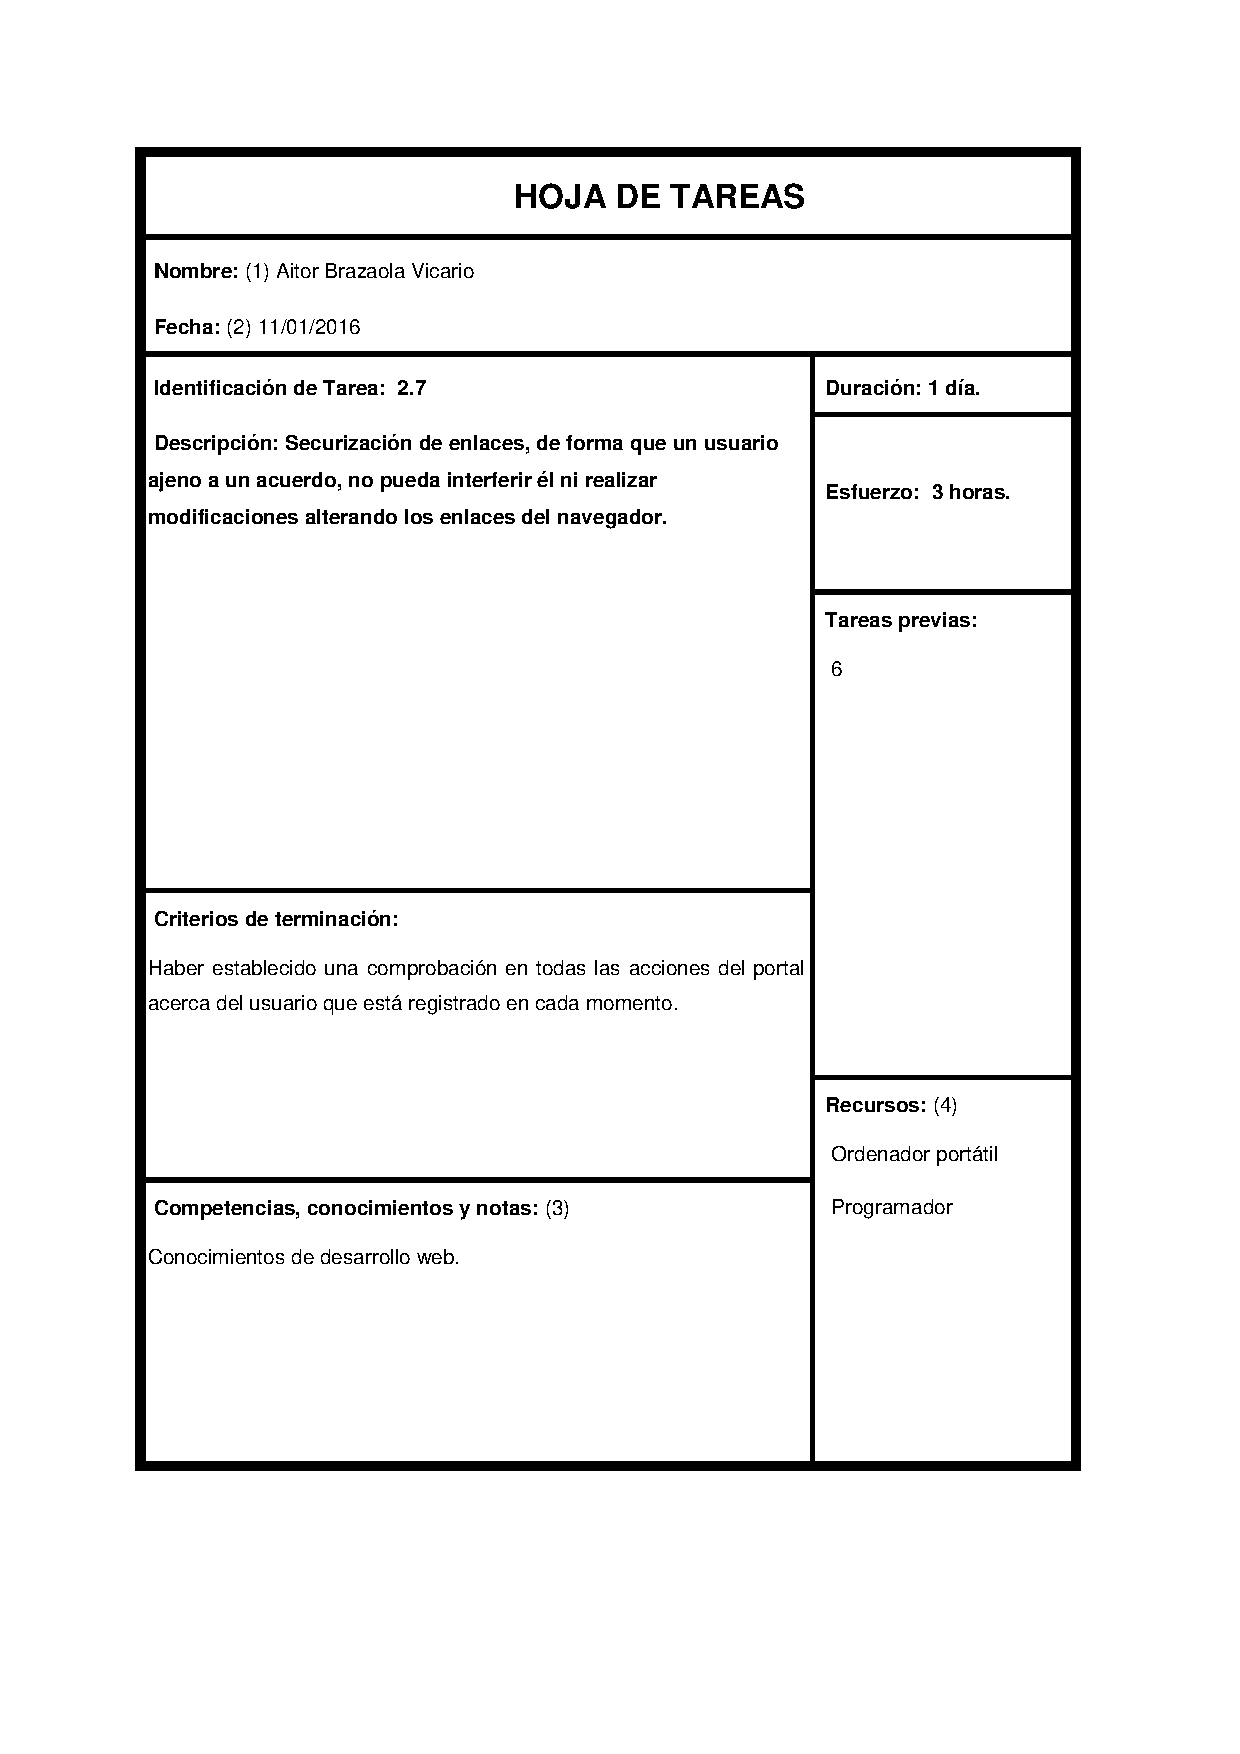
\includegraphics[width=0.9\textwidth]{fig/Tareas/27}
	\caption{Task 2.7.}
	\label{fig:t27}
\end{figure}

\begin{figure}[H]
	\centering
	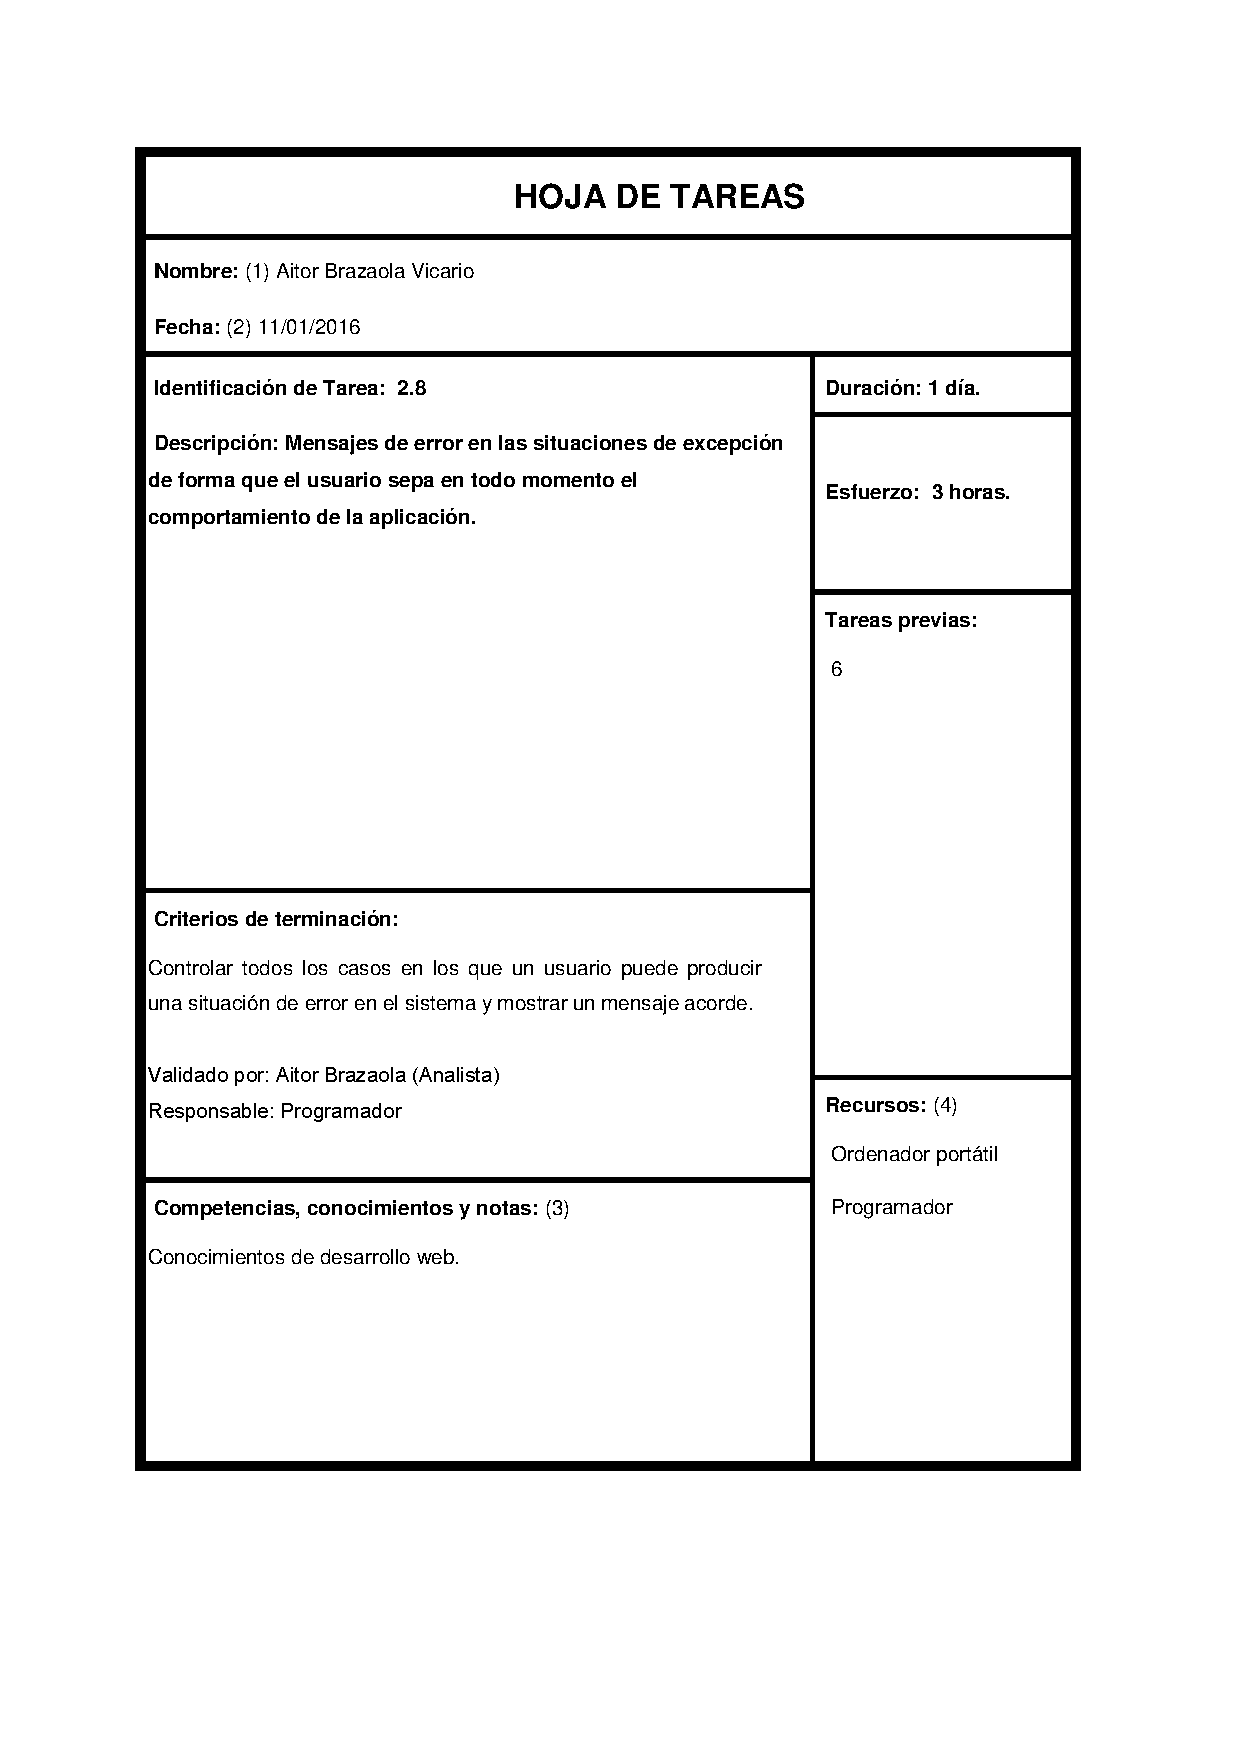
\includegraphics[width=0.9\textwidth]{fig/Tareas/28}
	\caption{Task 2.8.}
	\label{fig:t28}
\end{figure}

\begin{figure}[H]
	\centering
	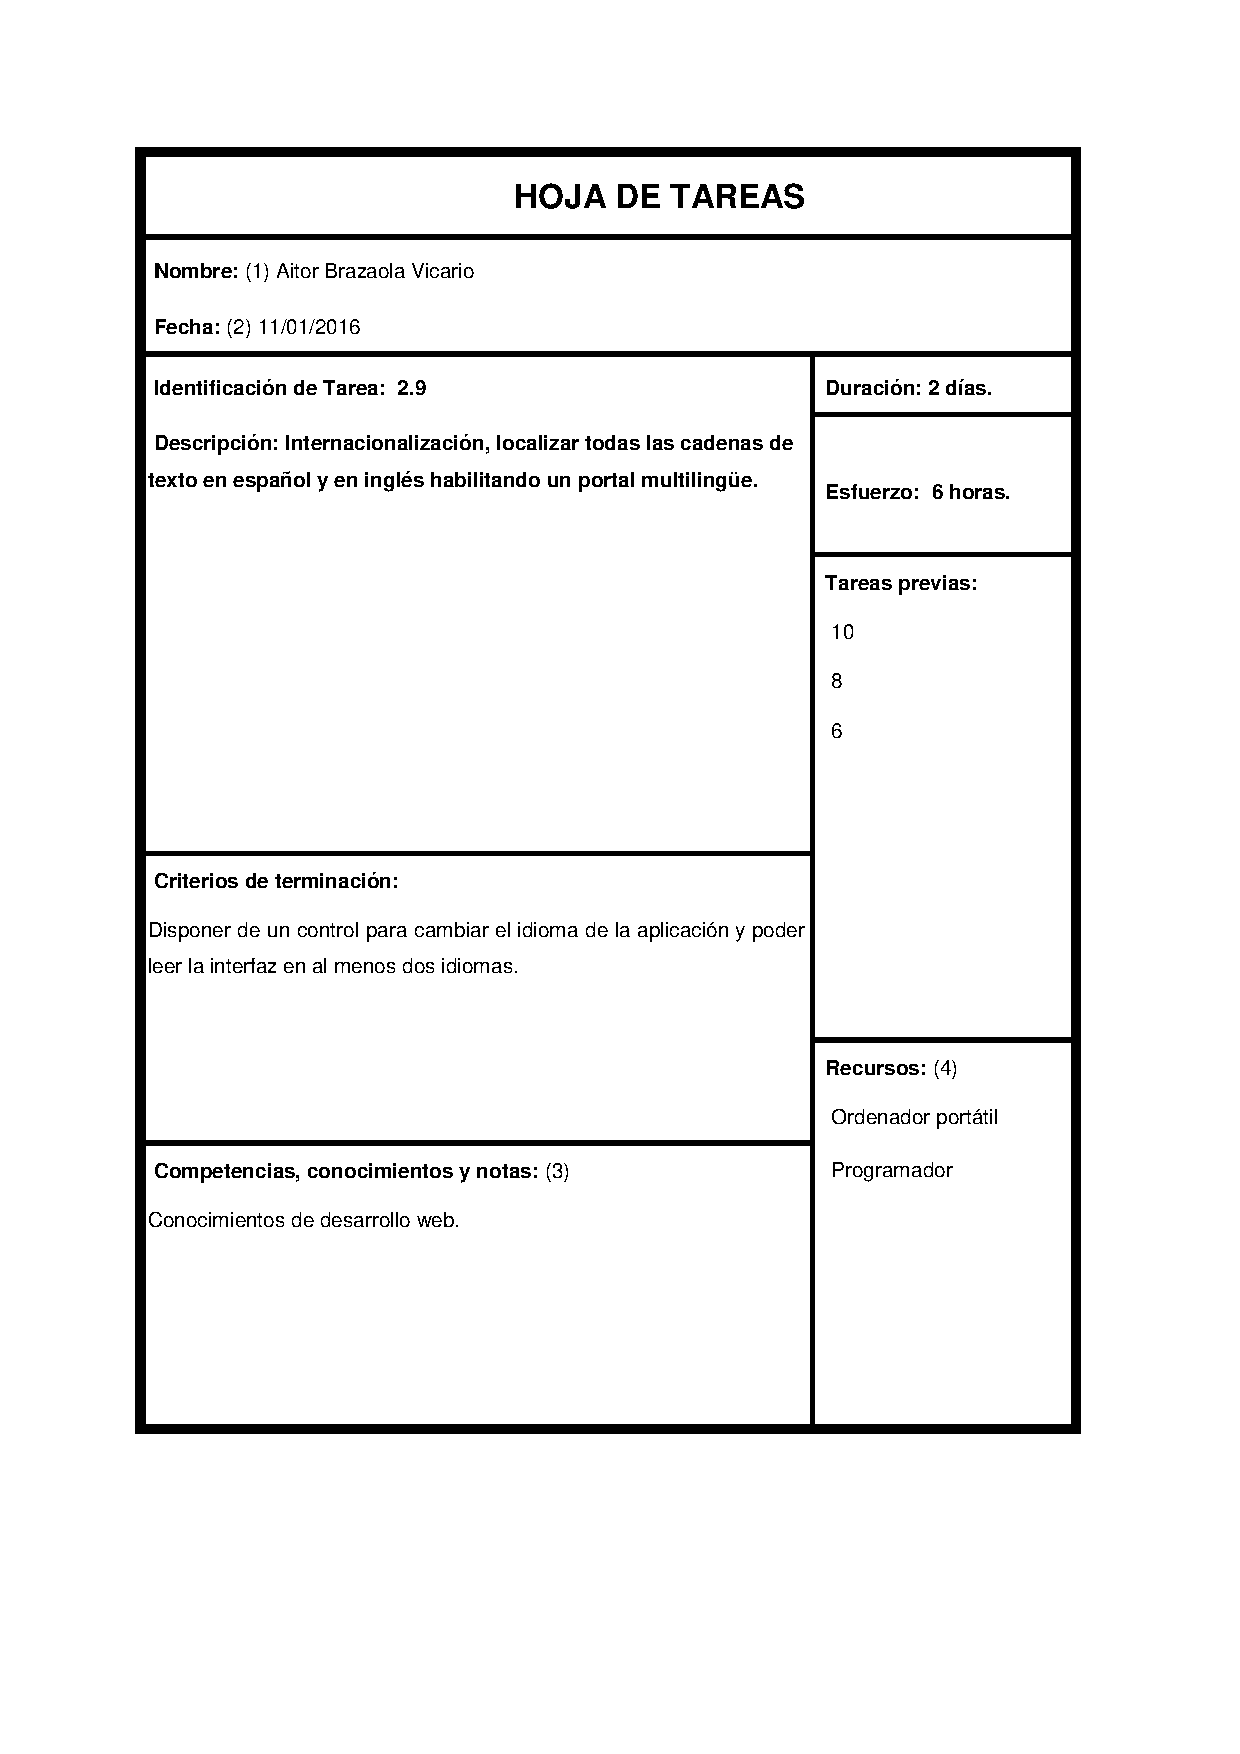
\includegraphics[width=0.9\textwidth]{fig/Tareas/29}
	\caption{Task 2.9.}
	\label{fig:t29}
\end{figure}

\begin{figure}[H]
	\centering
	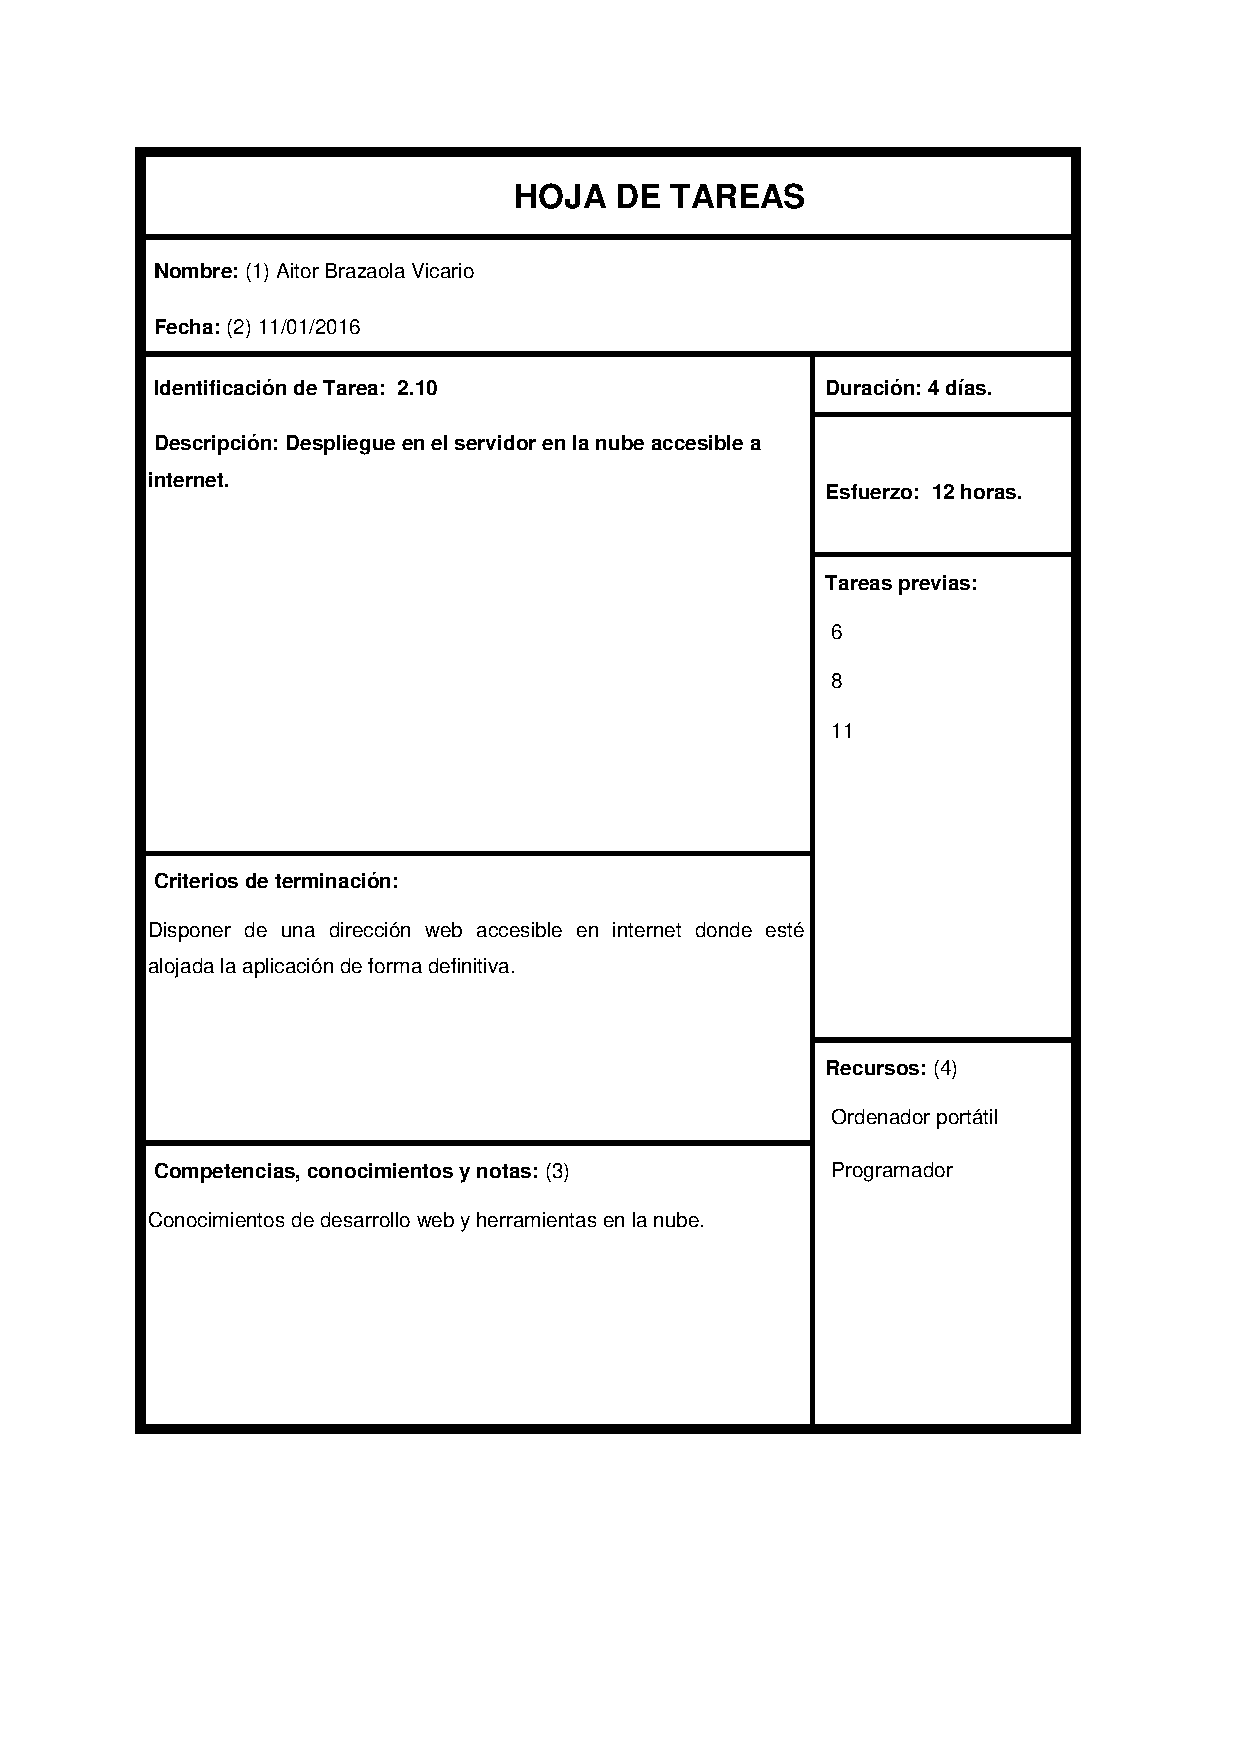
\includegraphics[width=0.9\textwidth]{fig/Tareas/210}
	\caption{Task 2.10.}
	\label{fig:t210}
\end{figure}

\begin{figure}[H]
	\centering
	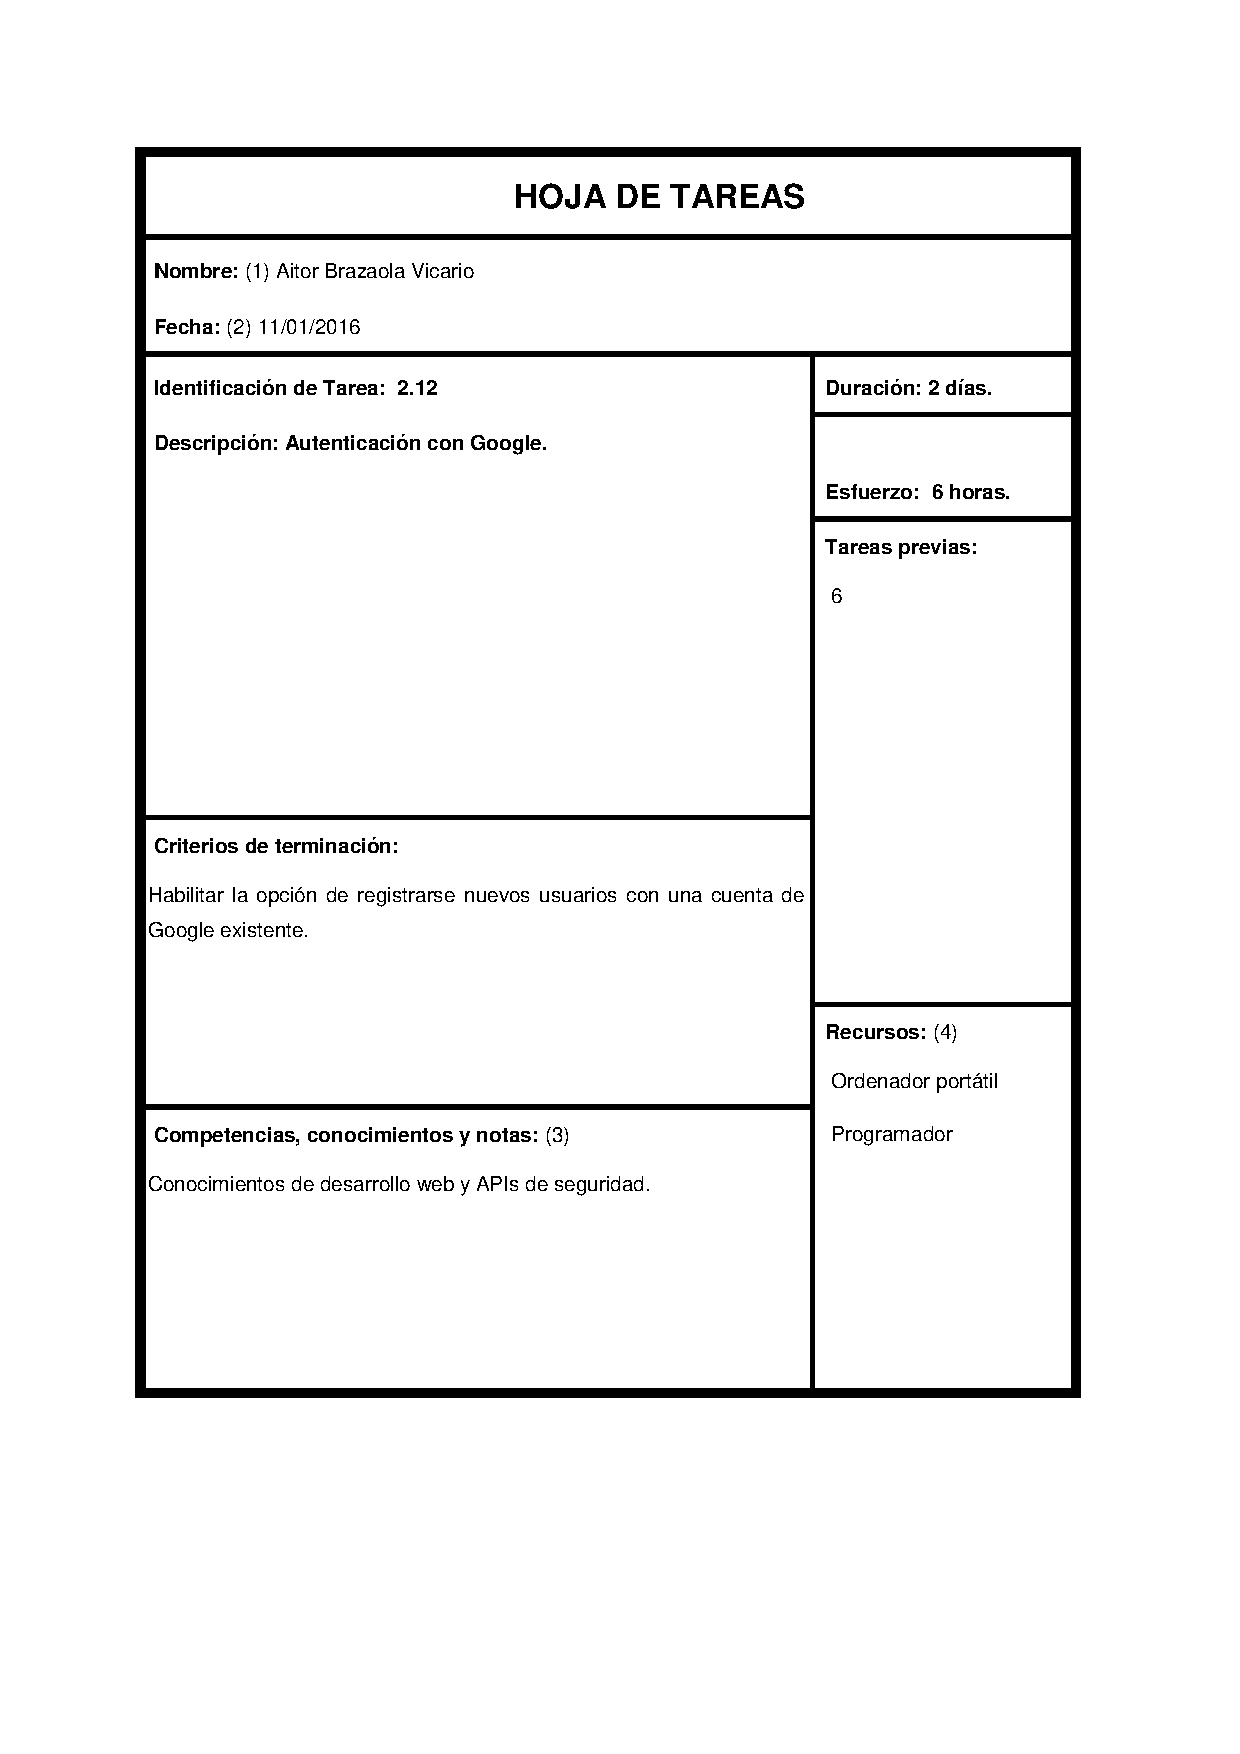
\includegraphics[width=0.9\textwidth]{fig/Tareas/212}
	\caption{Task 2.12.}
	\label{fig:t212}
\end{figure}

\begin{figure}[H]
	\centering
	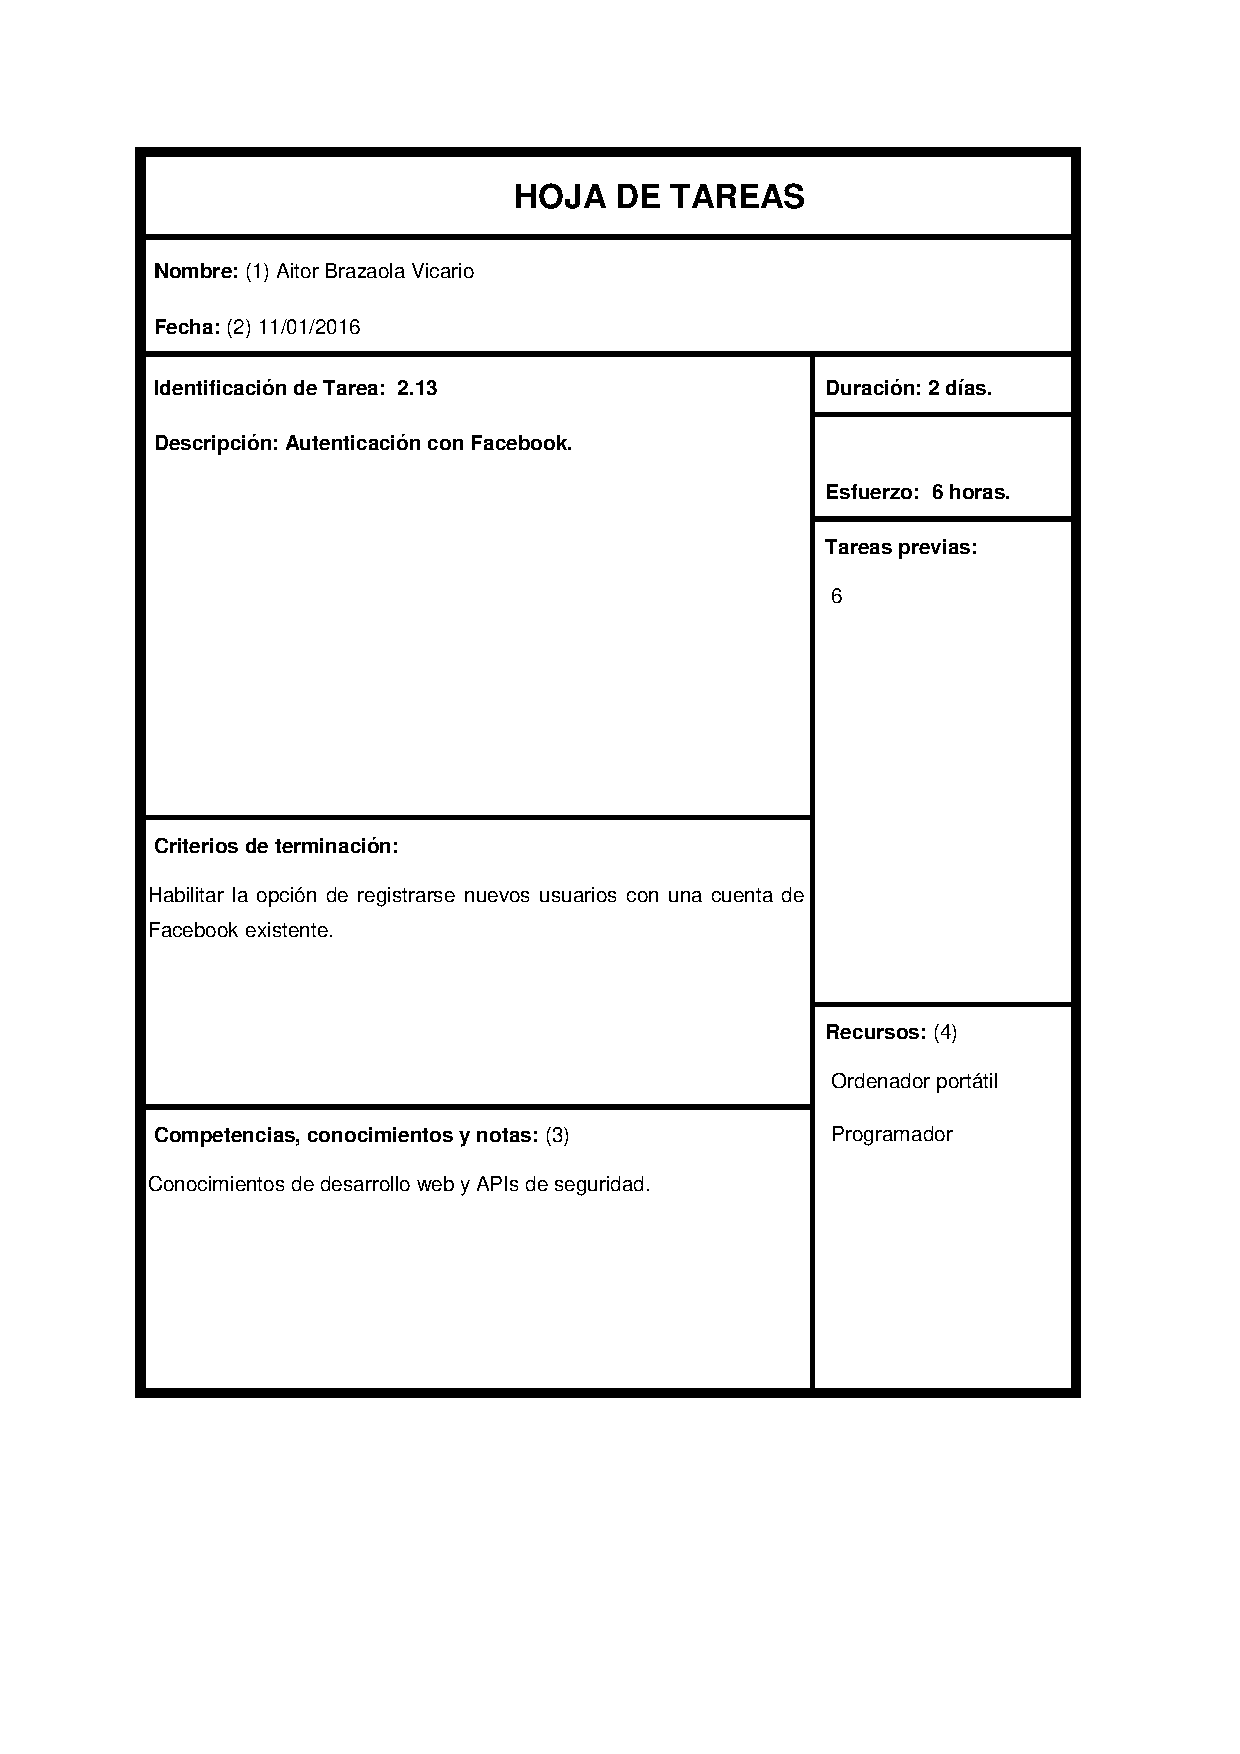
\includegraphics[width=0.9\textwidth]{fig/Tareas/213}
	\caption{Task 2.13.}
	\label{fig:t213}
\end{figure}

\begin{figure}[H]
	\centering
	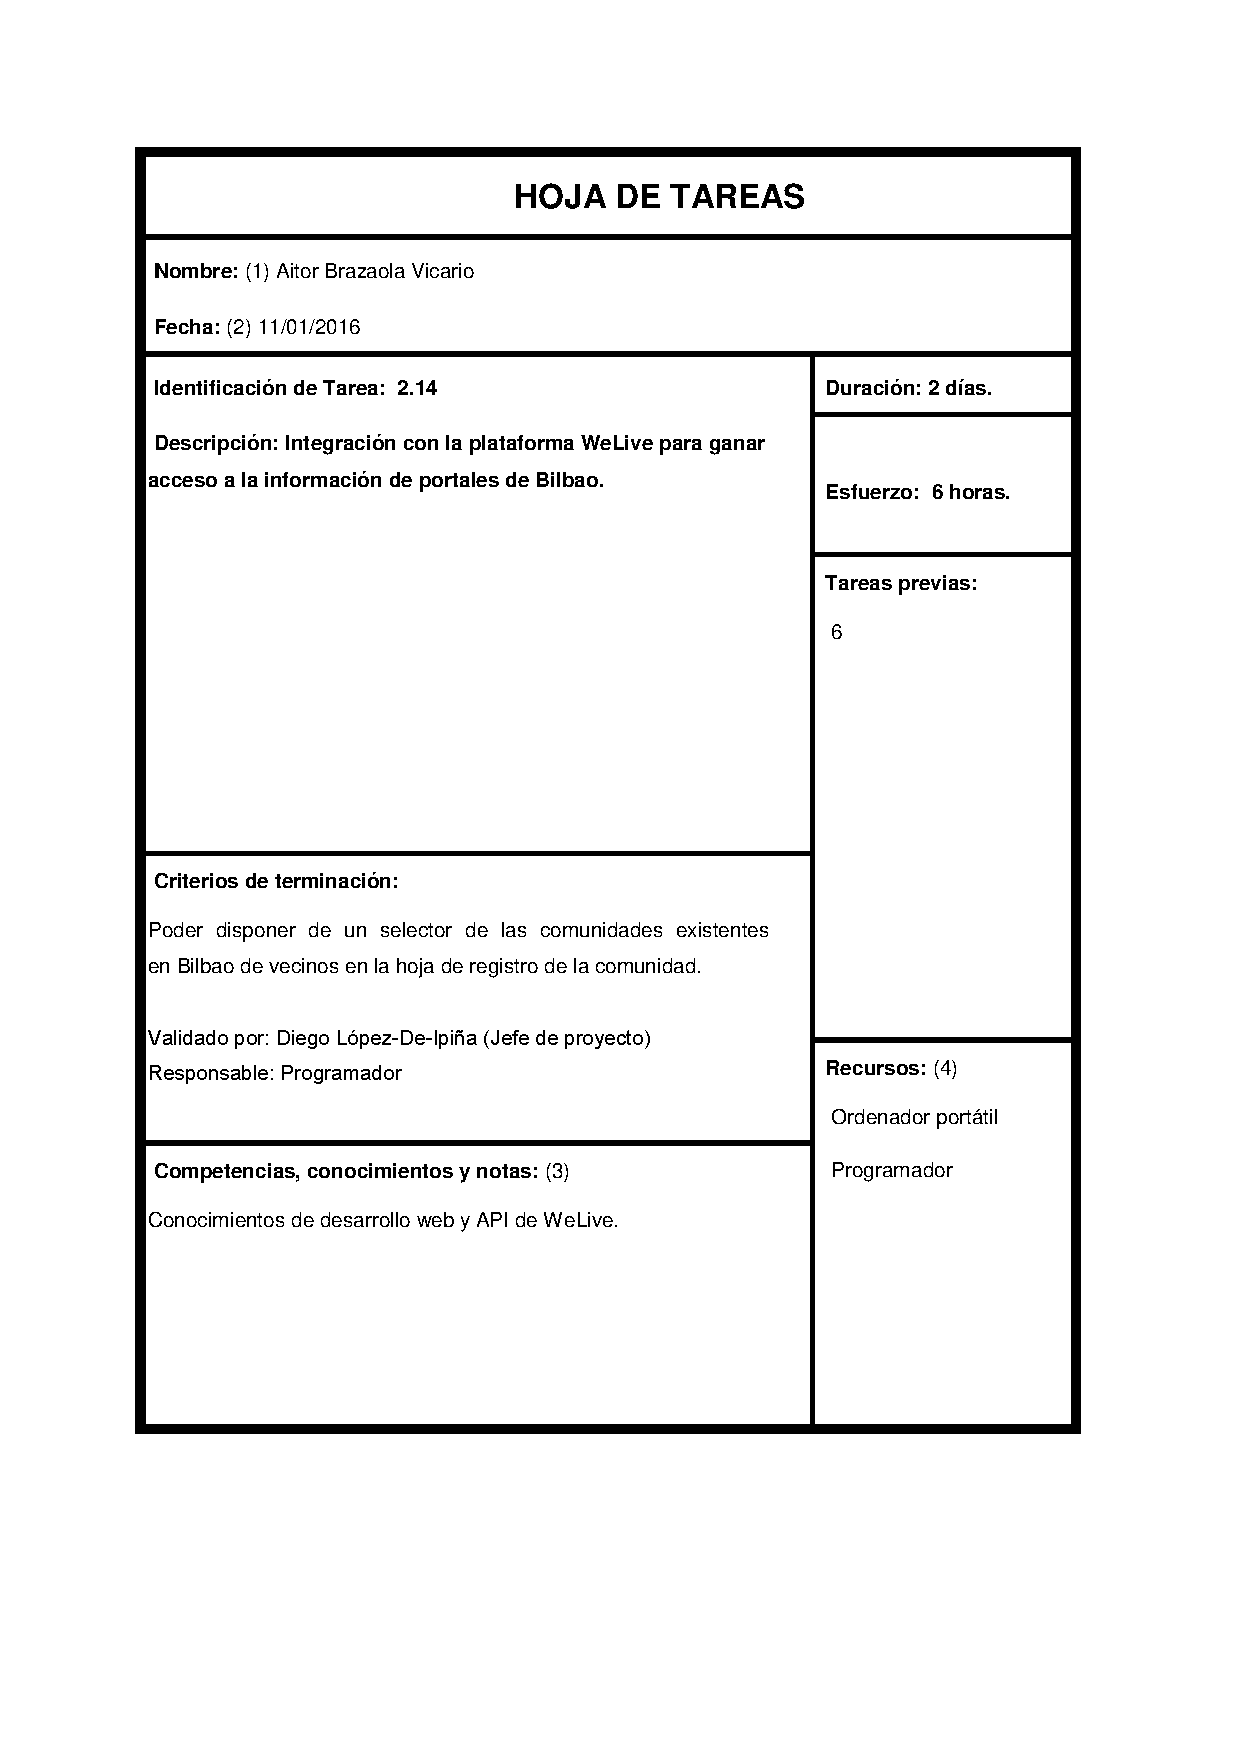
\includegraphics[width=0.9\textwidth]{fig/Tareas/214}
	\caption{Task 2.14.}
	\label{fig:t214}
\end{figure}

\begin{figure}[H]
	\centering
	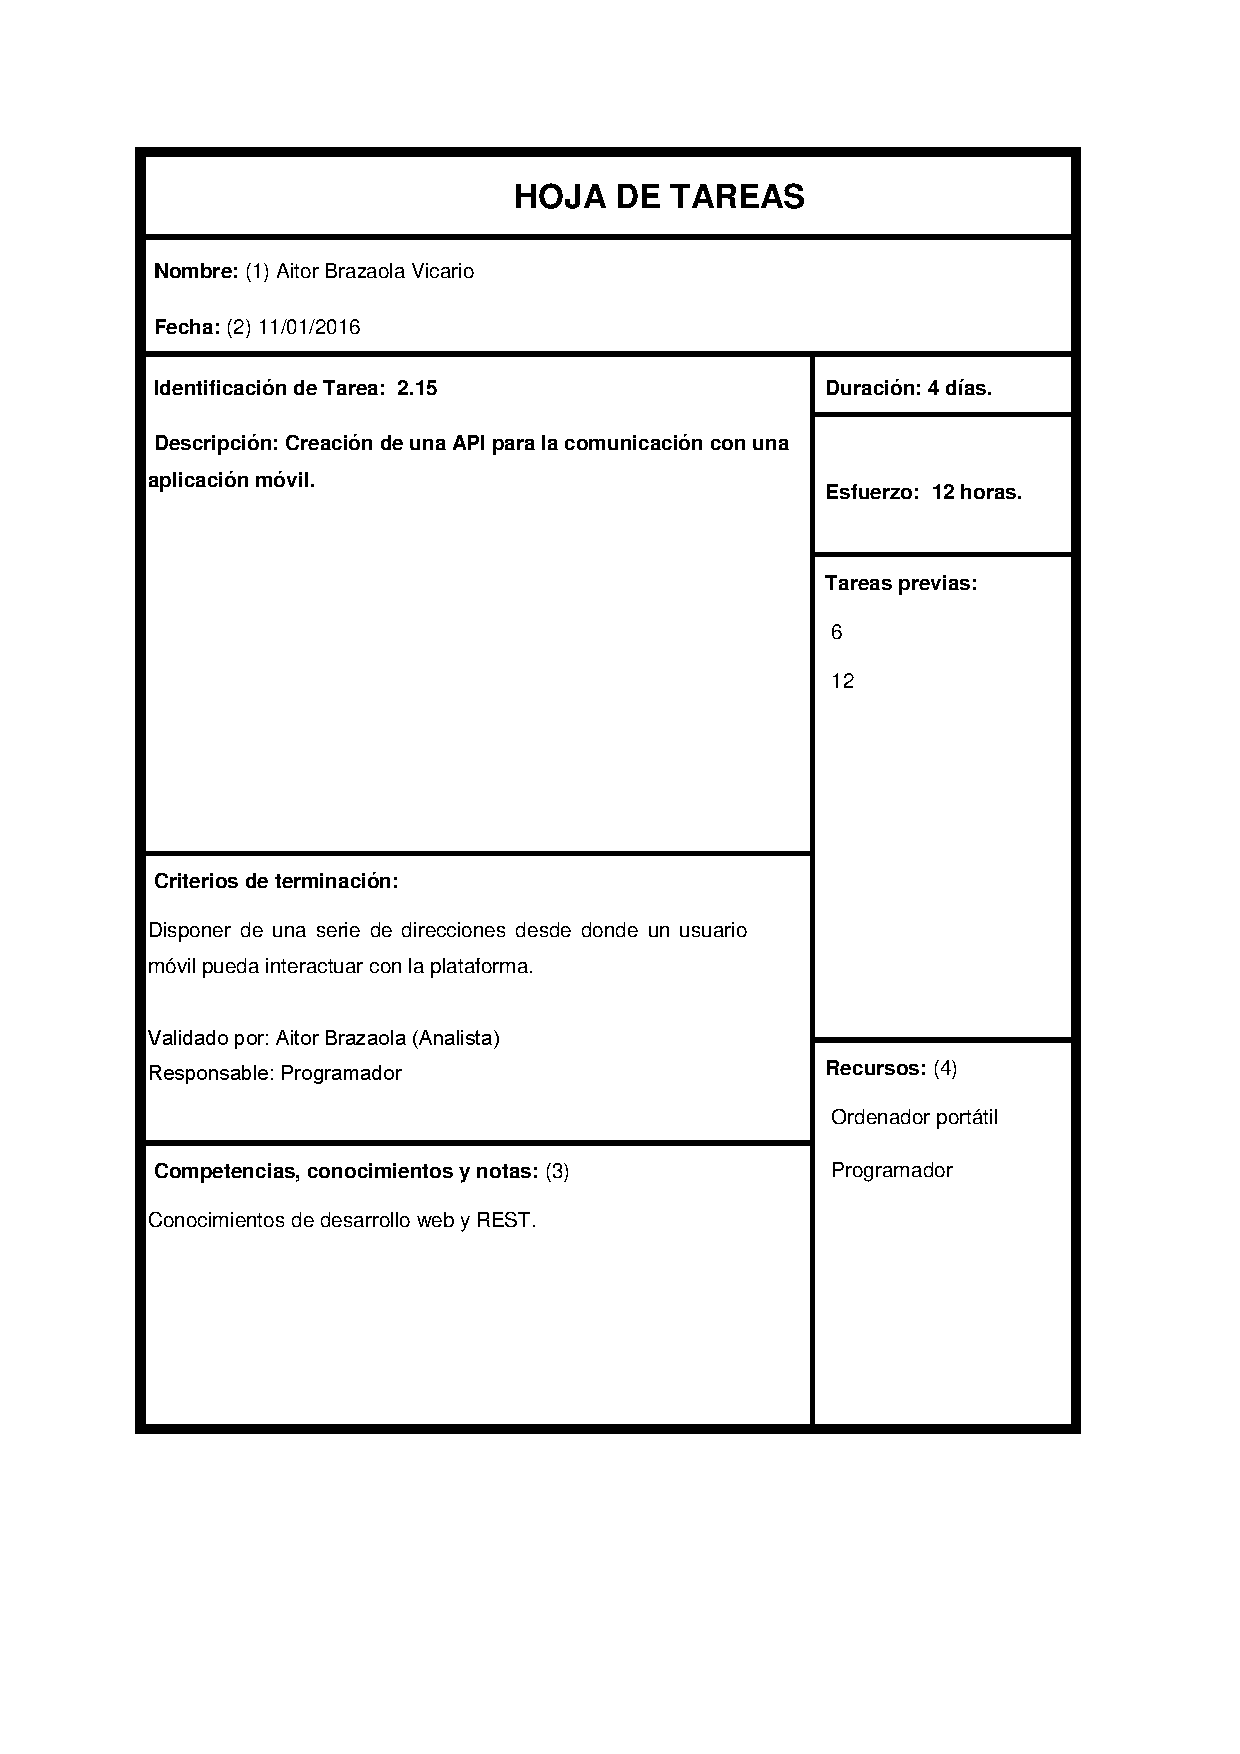
\includegraphics[width=0.9\textwidth]{fig/Tareas/215}
	\caption{Task 2.15.}
	\label{fig:t215}
\end{figure}

\begin{figure}[H]
	\centering
	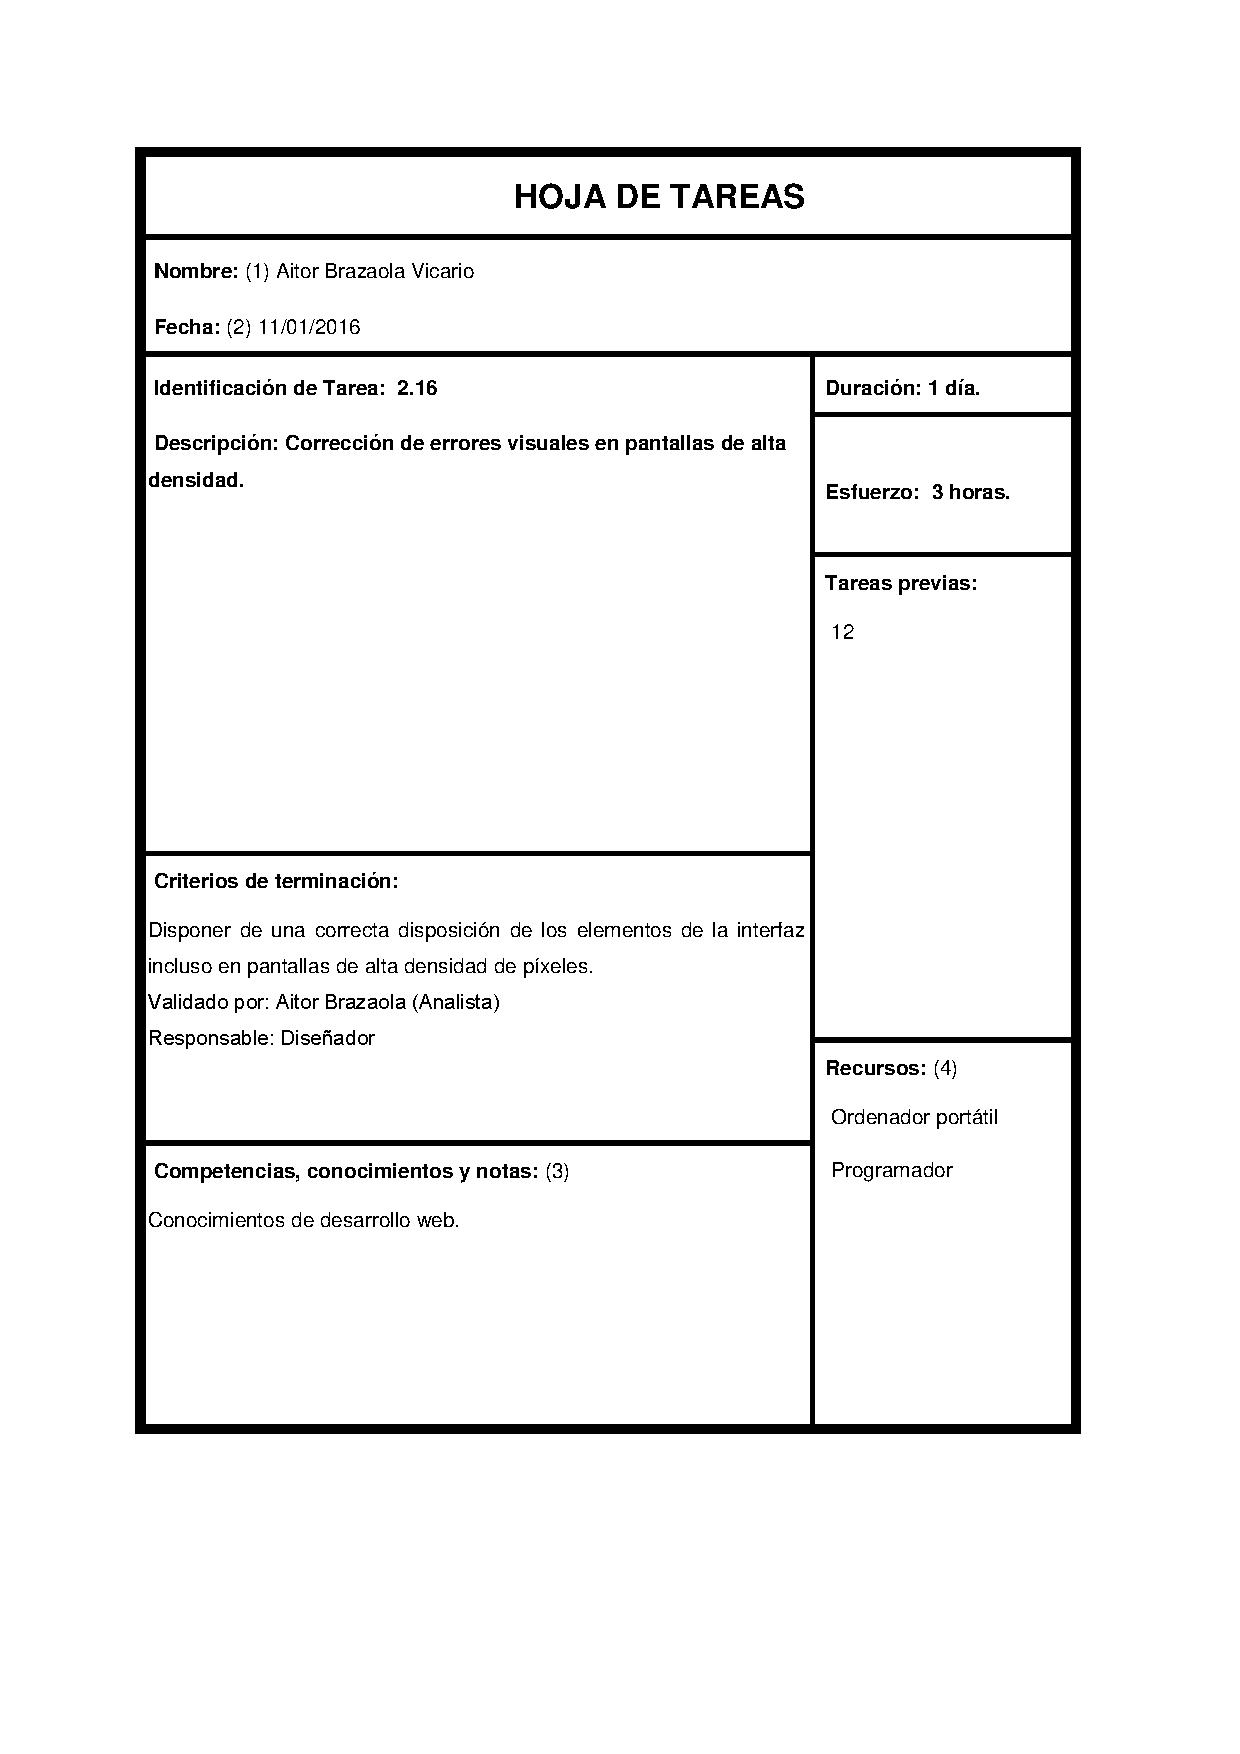
\includegraphics[width=0.9\textwidth]{fig/Tareas/216}
	\caption{Task 2.16.}
	\label{fig:t216}
\end{figure}

\begin{figure}[H]
	\centering
	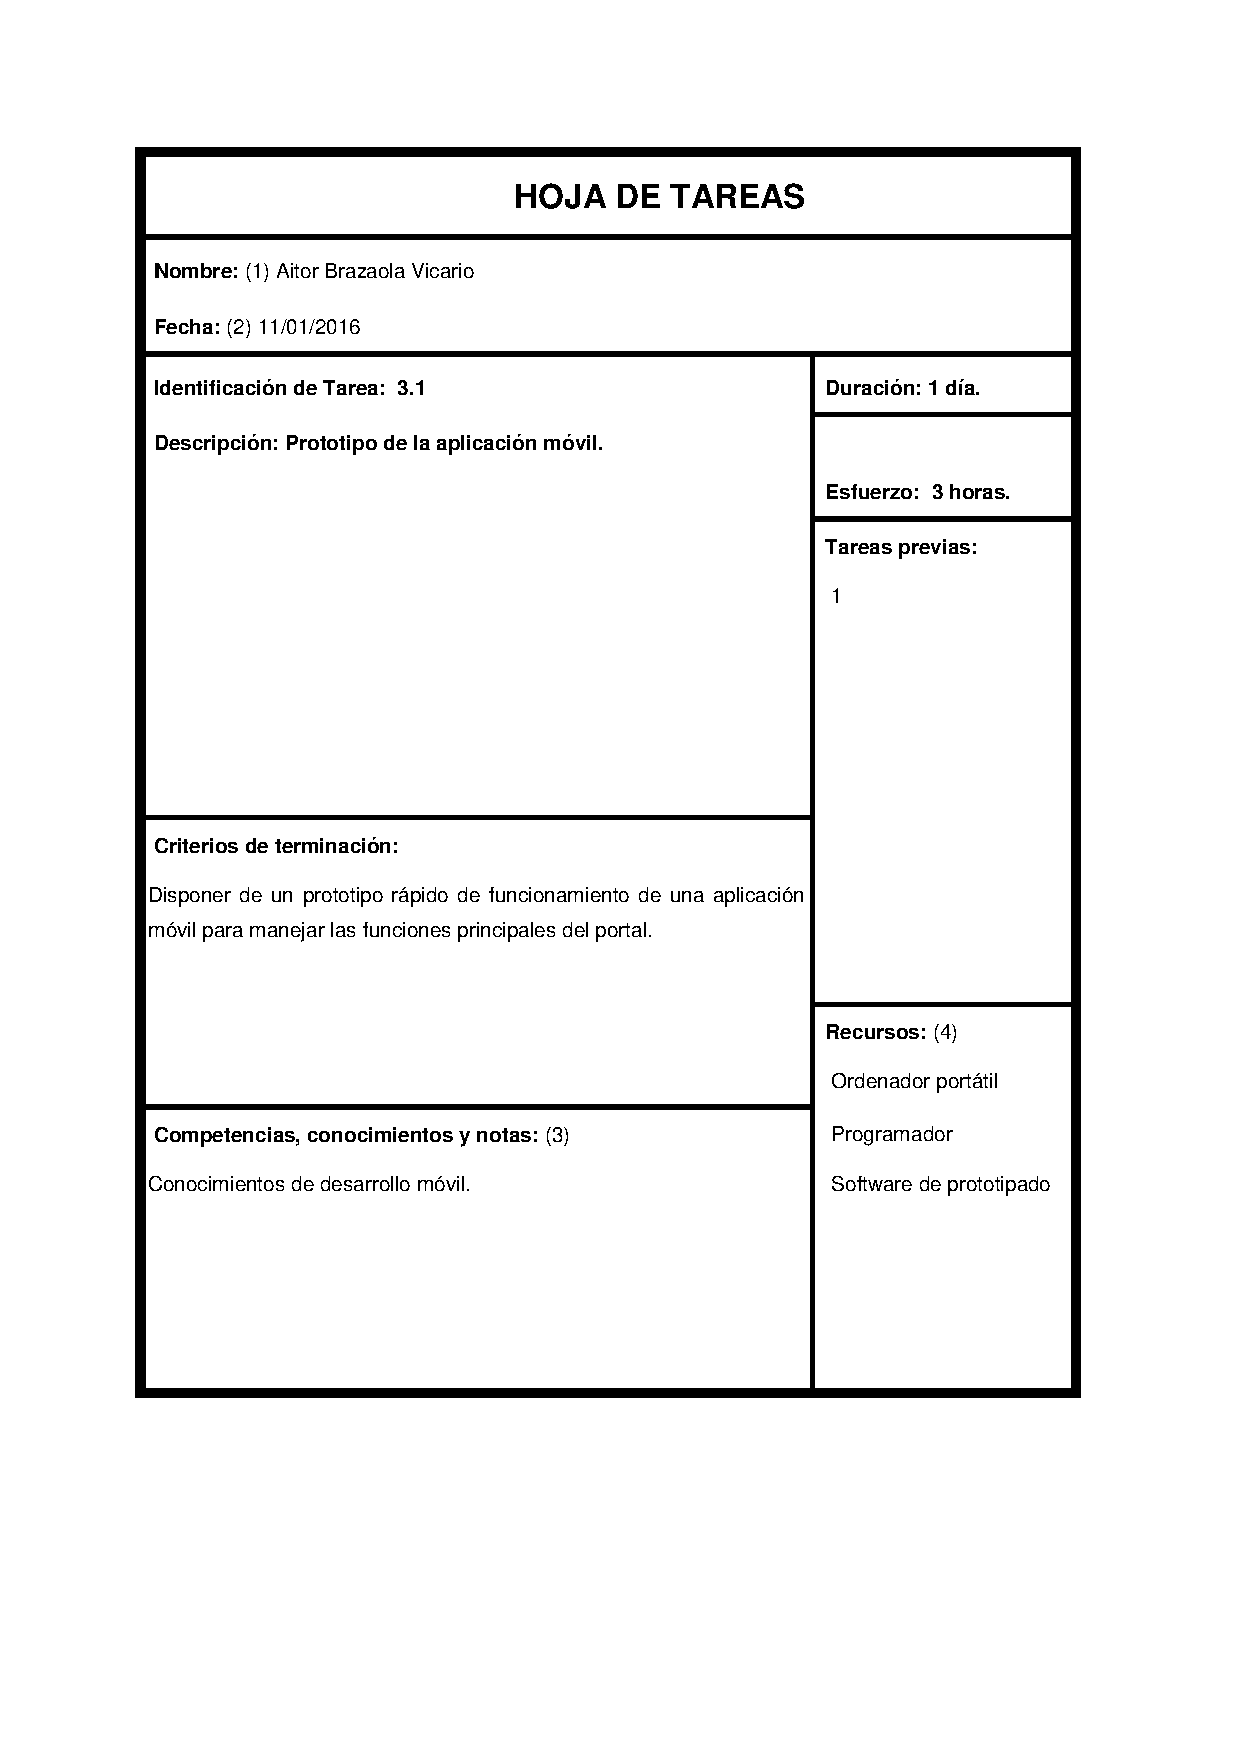
\includegraphics[width=0.9\textwidth]{fig/Tareas/31}
	\caption{Task 3.1.}
	\label{fig:t31}
\end{figure}

\begin{figure}[H]
	\centering
	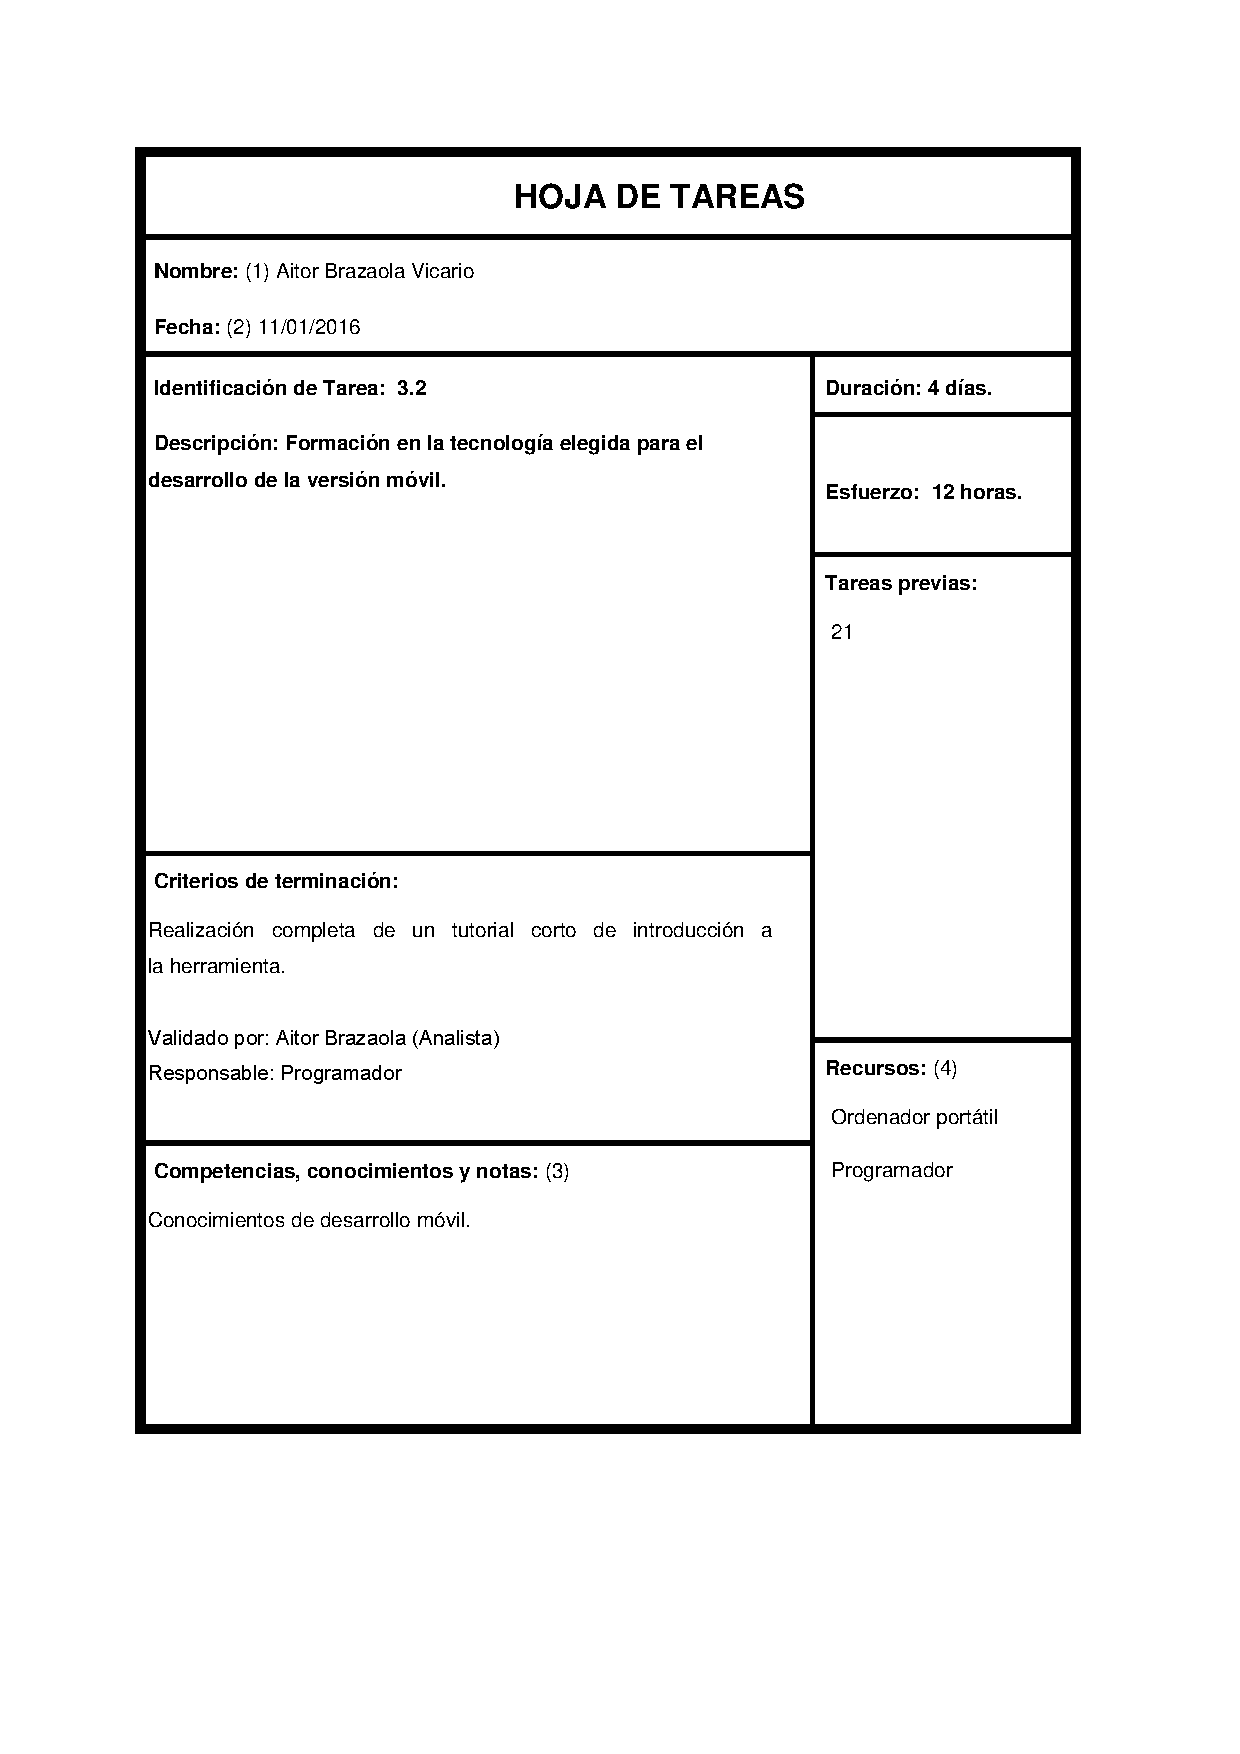
\includegraphics[width=0.9\textwidth]{fig/Tareas/32}
	\caption{Task 3.2.}
	\label{fig:t32}
\end{figure}

\begin{figure}[H]
	\centering
	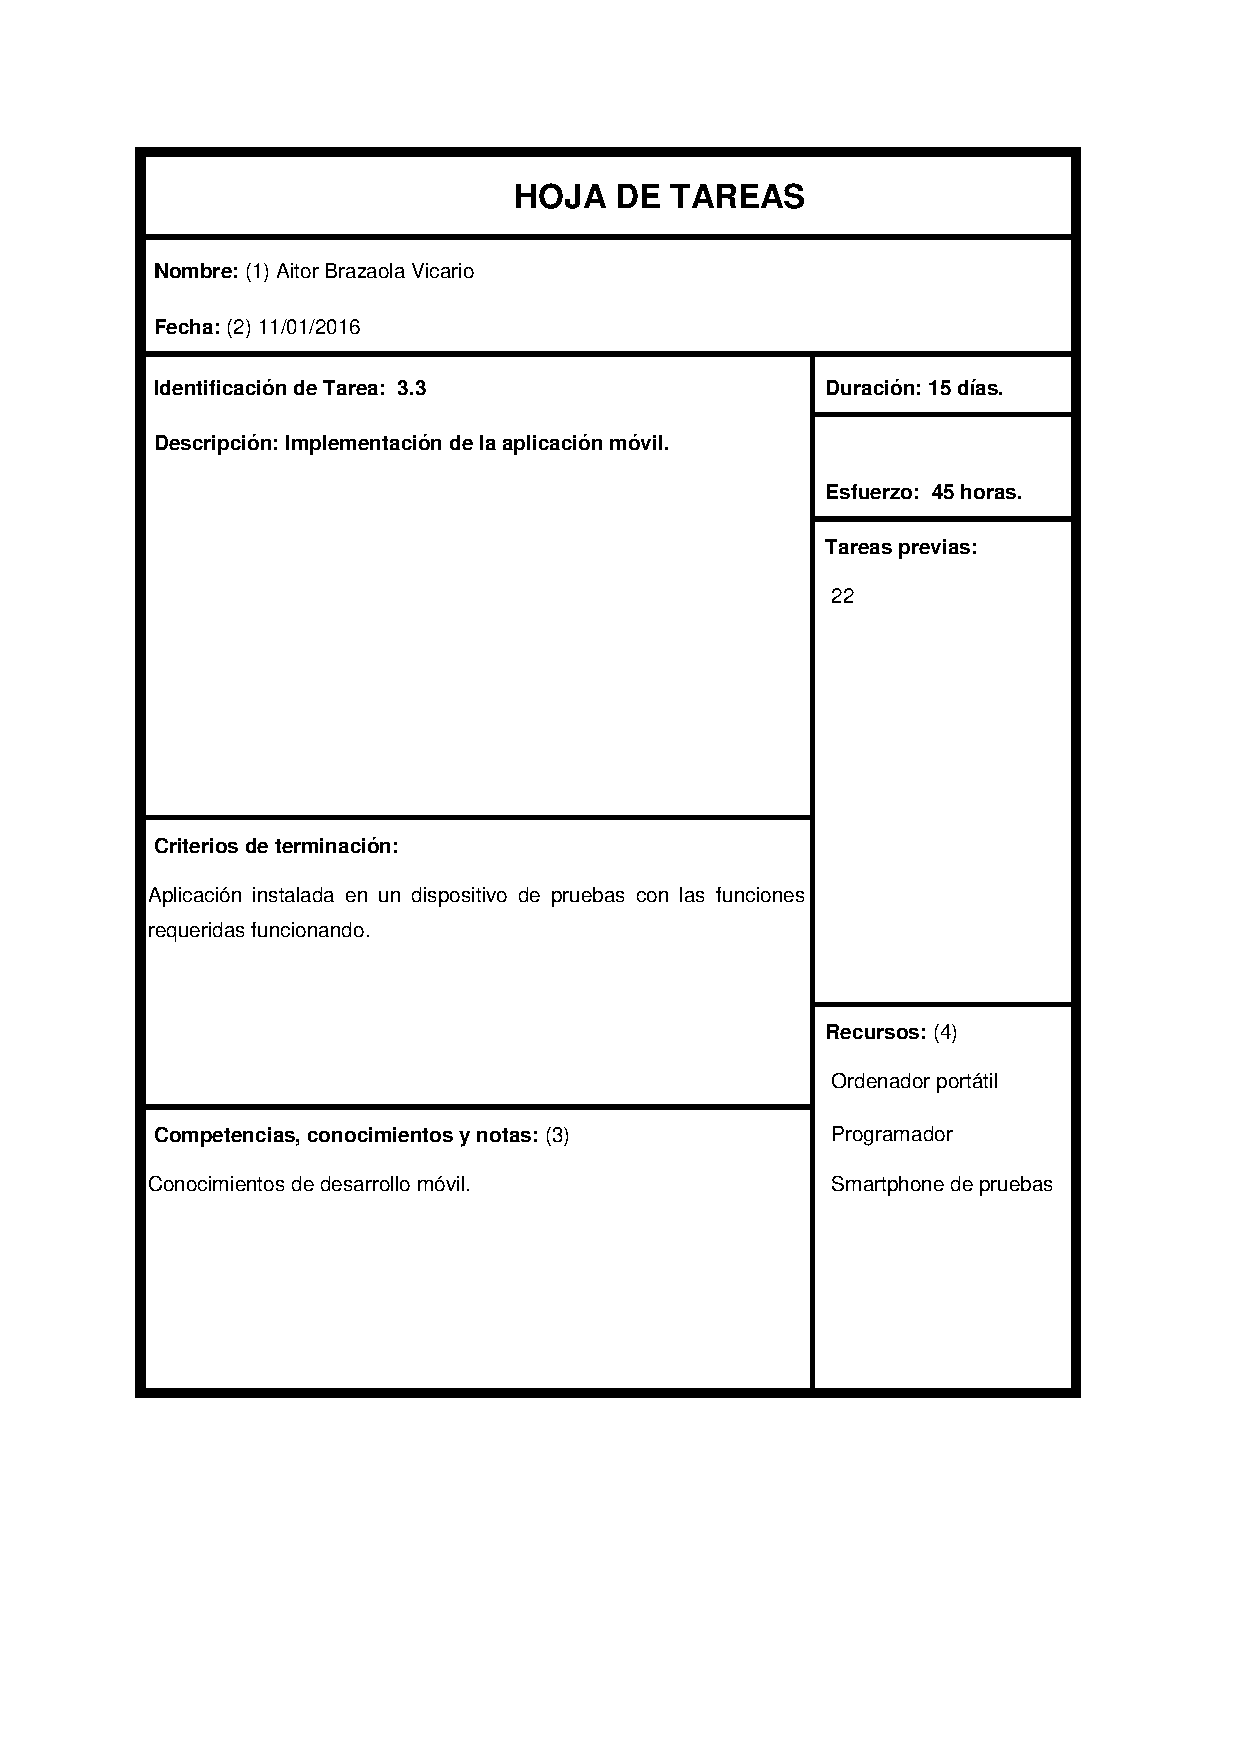
\includegraphics[width=0.9\textwidth]{fig/Tareas/33}
	\caption{Task 3.3.}
	\label{fig:t33}
\end{figure}

\begin{figure}[H]
	\centering
	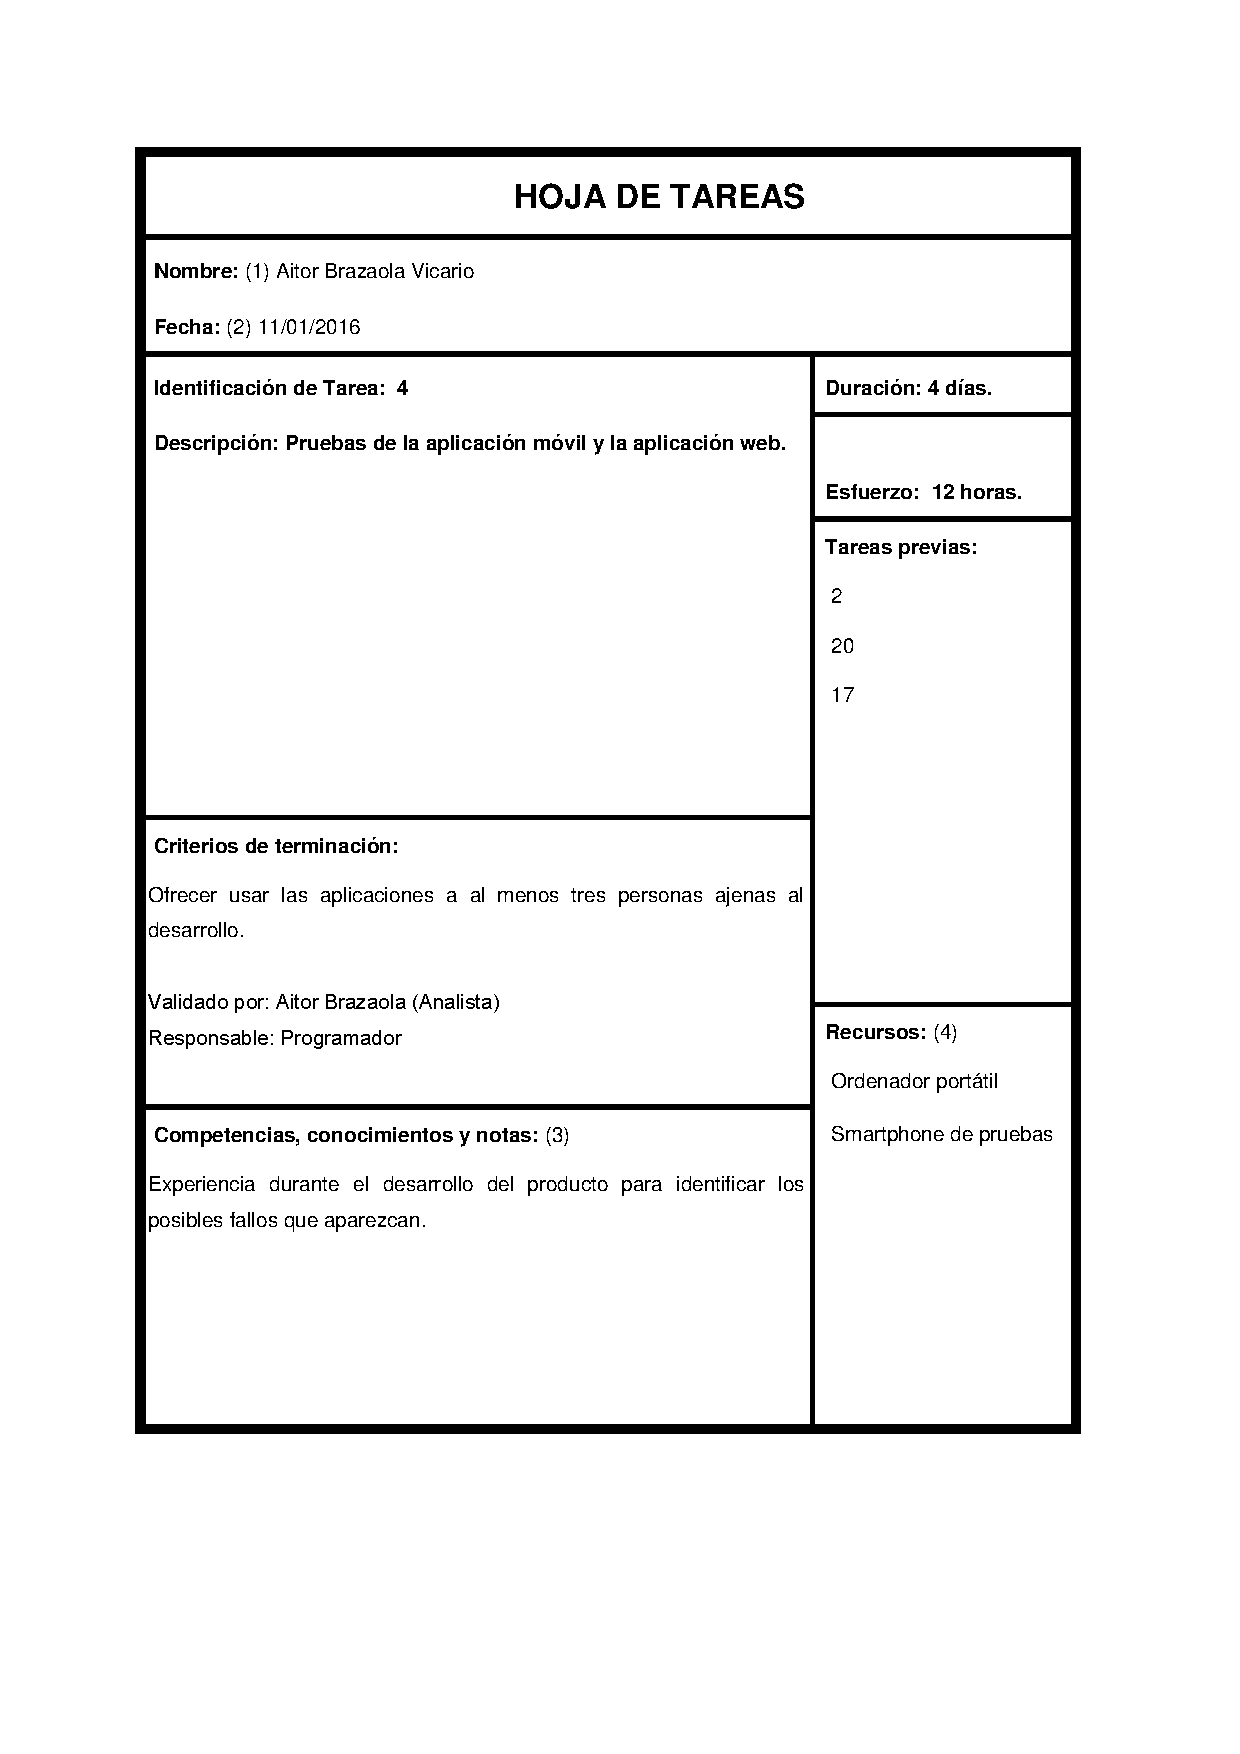
\includegraphics[width=0.9\textwidth]{fig/Tareas/4}
	\caption{Task 4.}
	\label{fig:t4}
\end{figure}
\section{Organization}
\subsection{Organizational structure}
The organization as can be seen in the figure \ref{fig:esquemaorganizacion}, is composed by the Project manager, and the student who perform the roles of programmer and designer.

\begin{figure}[h]
	\centering
	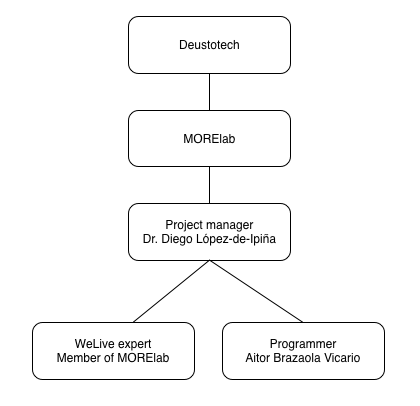
\includegraphics[width=0.7\linewidth]{fig/esquemaorganizacion}
	\caption[Organizational schema]{Organizational schema}
	\label{fig:esquemaorganizacion}
\end{figure}

Every two weeks there will be a session for reviewing the work done and the necessary changes will be assessed and if the product is already to consider as a functional unit.

\newpage
The main assistants will be the programmer and the project manager, the details exposed will be gathered in the meeting act, the template used for this proposal can be seen in the figure \ref{fig:Actareunion}, and will be prioritized over the rest of the features in the pipeline, avoiding develop in an incorrect way.

\begin{figure}[h]
	\centering
	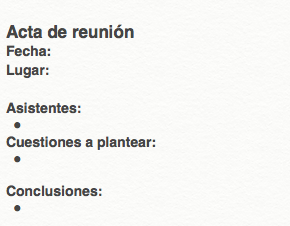
\includegraphics[width=0.7\linewidth]{fig/Actareunion}
	\caption[Template meeting act]{Template meeting act}
	\label{fig:Actareunion}
\end{figure}
\subsection{Human resources plan}
The student will be the unique physical person in the development team but will be necessary the acquisition of various roles along the project, it is true that un punctual cases can be helped by other mates of the laboratory where is working on, but the most of the project is developed by him.

Following, there are listed the main roles played by the student:

\begin{description}
	\item[Programmer:] It is responsible for creating all the logic of the program and perform the different configurations in the devices responsible for the platform work. Its functions also cover the early stages of software design, data schema creation and conduct appropriate tests to detect errors.
	
	\item[Designer:] It is commissioned to design a user interface that fits all available screens and make the application accessible to people with disabilities and ensure a satisfactory user experience and consistent navigation between different sections of the web.
\end{description}

In addition to the student, the project has its project manager who is responsible for approving all changes and proposals that the student considers interesting to improve the product, will be present at the meetings and will be responsible for marking the milestone dates.

\chapter{Planning}\label{cha:planning}
\section{Precedence diagram}
\begin{figure}[H]
	\centering
	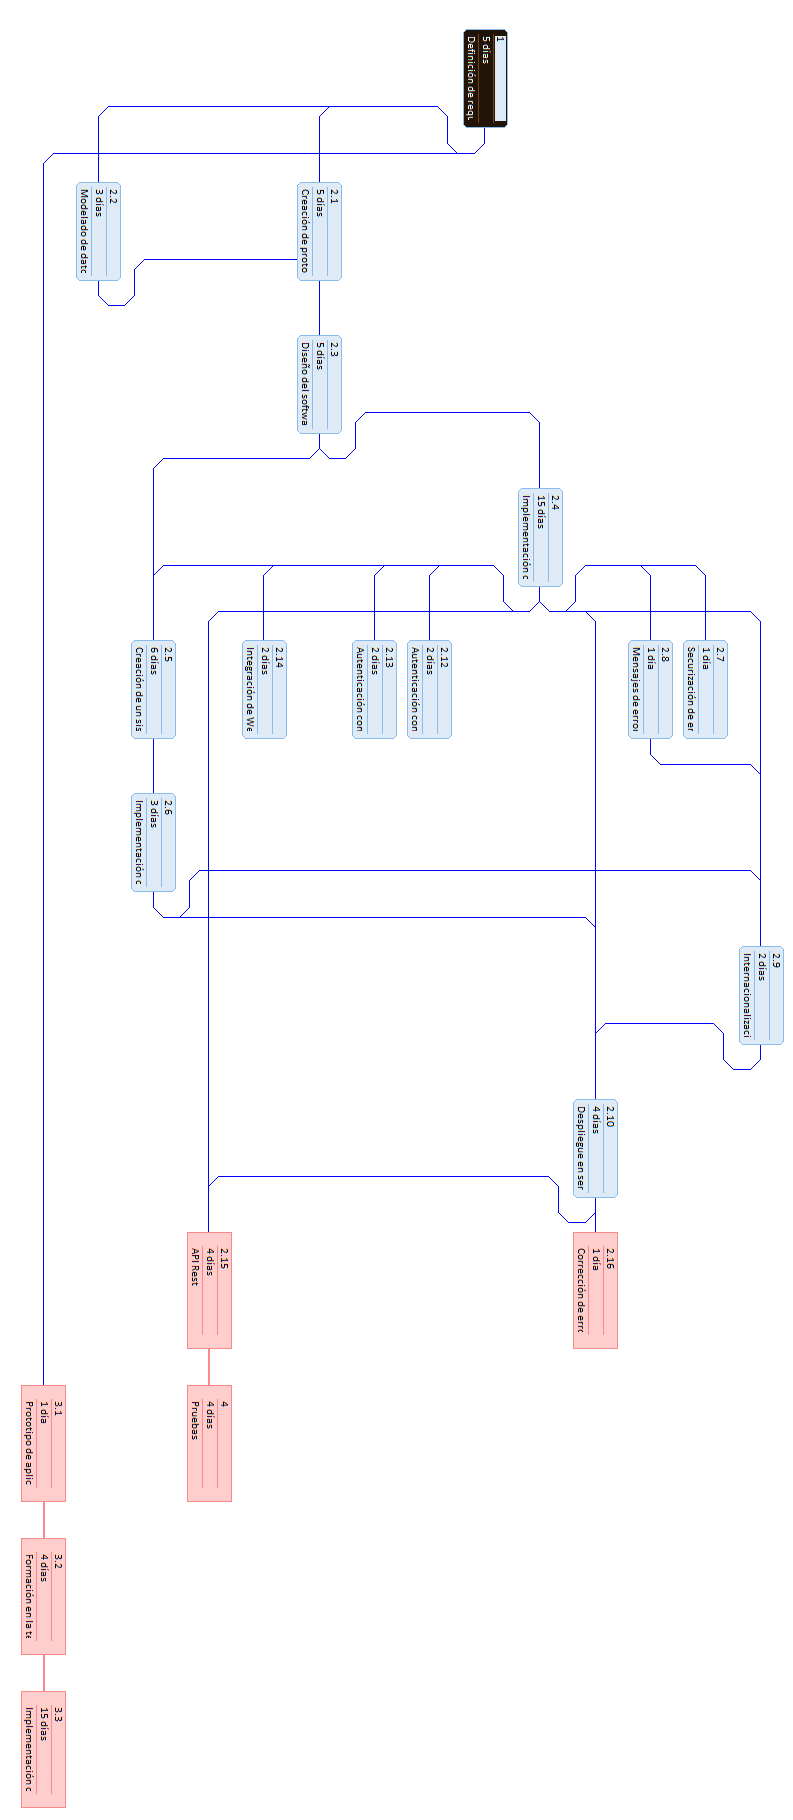
\includegraphics[width=210pt]{fig/precedencia}
	\caption{Precedence diagram}\label{fig:precedencediagram}
\end{figure}

The project development is going to happen during the working time in DeustoTech MORElab of 4 daily hours, and the team will be formed by the following actors:

\begin{description}
	\item[Programmer:] Person in charge of programming the control structures of the platform.
	\item[Designer:] Person in charge of the final appearance with the end user will interact.
	\item[Project manager:] Person in charge of monitoring the progress of the project and its organization.
	\item[Experto en plataforma WeLive:] MoreLab team member participating in the development of technical advice WeLive platform for the team.
\end{description}

\newpage
\section{GANTT diagram}
\begin{figure}[H]
	\centering
	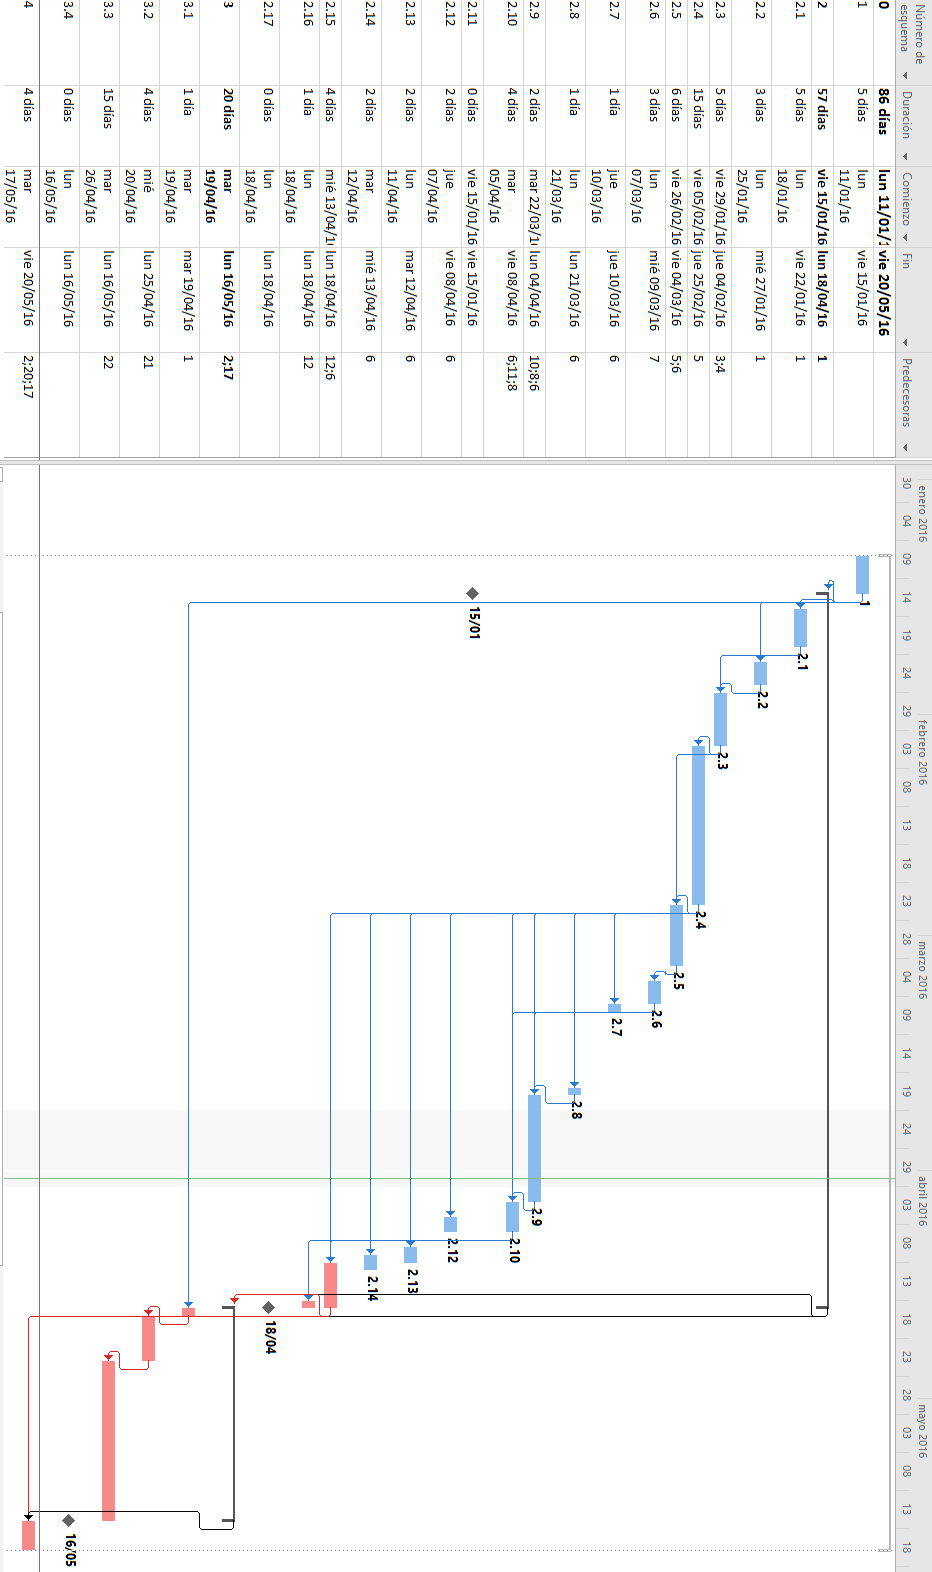
\includegraphics[width=340pt]{fig/gantt}
	\caption{GANTT diagram}\label{fig:gantt}
\end{figure}

\section{Workload estimation by profile}
The following estimation is based on the different profiles of the total 255 hours:
\begin{description}
	\item[Programmer:] 215 hours.
	\item[Designer:] 22 hours.
	\item[Project manager:] 15 hours.
	\item[WeLive platform expert:] 3 hours.
\end{description}

\begin{itemize}
	\item 1. Requirements definition: 15 hours.
	\item 2. Web application: 168 hours.
	\begin{itemize}
		\item 2.1. Web application prototype: 15 hours.
		\item 2.2. Data modeling: 9 hours.
		\item 2.3. Software design: 15 hours.
		\item 2.4. Implementation of the core features: 51 hours.
		\item 2.5. Users system creation: 18 hours.
		\item 2.6. Implementation of mail notifications: 15 hours.
		\item 2.7. Link security checks: 3 hours.
		\item 2.8. Friendly error messages: 3 hours.
		\item 2.9. Internationalization: 6 hours.
		\item 2.10. Server deployment: 12 hours.
		\item 2.13. Visual customization and logo: 6 hours.
		\item 2.14. WeLive API integration: 12 hours.
		\item 2.16. High density displays visual fixes: 3 hours.
	\end{itemize}
	\item 3. Mobile application: 60 hours.
	\begin{itemize}
		\item 3.1. Mobile application prototype: 3 hours.
		\item 3.2. Learning the selected technology for development: 12 hours.
		\item 3.3. Mobile app implementation: 45 hours.
	\end{itemize}
	\item 4. Tests: 12 hours.
\end{itemize}
\chapter{Budget}\label{cha:budget}
The budget will take into account only the hours of work because the necessary equipments are already owned by the programmer and DeustoTech facilities where the project is located.

\begin{table}[H]
	\centering
	\caption{Budget by profile.}\label{tab:budgetprofile}
	\begin{tabular}{cccc}
		\toprule
		\textbf{Profile} & \emph{Workload} & \emph{Cost} & \emph{Price}\\
		\midrule
		Programmer  & 255 h.     & 9€/h. & 2295€ \\
		Designer   & 22 h.     & 9€/h. & 198€ \\
		Project manager & 12 h.     & 50€/h.  & 600€ \\
		WeLive platform expert & 3 h.     & 6€/h. & 18€ \\
		TOTAL & & & 3.111€\\
		\bottomrule
	\end{tabular}
\end{table}

\chapter{Development}\label{cha:development}
The main section of the development is going to be for the web application, the part of the project with more effort, and technologies involved in development, then, the mobile application as a derivative product from the web app will be explained in detail reasoning the technologies used with their advantages and drawbacks.

Both products has been submitted to testing with collaborators and the process of the tests will be detailed, finally a user manual will be included for helping to use all functionality implemented by the platform.
\section{Web application}
\subsection{Software and Hardware requeriments}
The application must have a good user interface, allowing users from all ages for using it with less effort, furthermore, the application must make a good usage of the public data of the Bilbao's council provide using WeLive platform.

\subsubsection{Software requirements}
\begin{itemize}
	\item All communities existing on Bilbao must be available for register in the platform.
	\item The communities must have a common place to exchange information among members.
	\item The users information must be protected with security measurements for avoiding data stealing or spam.
	\item Users can post or attend offers among them.
	\item Users can post or attend requests among them.
	\item Users can set an access password to communities for avoid external viewers.
	\item Users can belong to more than once community.
	\item There have to exist a way for measure the trustfulness of each user in the community, a reputation system.
	\item There have to exist a mail notification system in real time for the activity in each community.
	\item The look and feel of the platform should fit to different sizes of screen.
\end{itemize}

\subsubsection{Hardware requirements}
\begin{itemize}
	\item The application must run on MORElab servers.
	\item The performance of the application must be smooth and fast on every web browser.
	\item The platform must have a smartphone application.
	\item The platform must be able to manage a huge quantity of request concurrently with no fault.
	\item No new hardware than the already existing on MORElab must be need.
\end{itemize}
\subsection{Hardware specification}
For fulfilling the previous requirements and taking advantage of the web server technology already available on MORElab, the server where the application is deployed belongs to the laboratory and the same domain of MORElab applications is used. The application is accessible on http://apps.morelab.deusto.es/auzonet

The hardware requirements are going to fit the existing hardware shared for other applications developed on MORElab, specifically, in the server called "Olentzero" with the following specifications:

\begin{itemize}
	\item Intel(R) Xeon(R) CPU E5-2430 @ 2.20GHz
	\item 16 GB RAM
	\item 1TB Hard disk
\end{itemize}

Deploying here the application where already have available a complete software environment of web dependencies save time reusing already existing modules.

\subsection{Software specification}
The web application running on "Olentzero" server must have the following software installed for correct performance:

\begin{description}
	\item[Ubuntu Server 14.04.4 LTS:] Open Source operating system running on "Olentzero" server.
	\item[Python 2.7 or newer:] Python is a widely used high-level, general-purpose, interpreted, dynamic programming language.
	\item[Django framework 1.9:] Develop the web application
	\item[gunicorn:] Python WSGI HTTP server for UNIX to serve the web application
	\item[nginx:] A free, Open-Source, high-performance HTTP server and reverse proxy for serve the static and media files.
	\item[pip:] A python package manager for install python packages in the virtual environment.
	\item[supervisord:] A client/server system to monitor and control processes on UNIX-like operating systems for monitoring the gunicorn instance that serves the web application.
	\item[virtualenv:] A tool to create isolated python environments for create an isolated environment for developing and deploying purposes, without library conflicts.
	\item[virtualenvwrapper:] A set of extensions to virtualenv for ease the use of virtualenv through the command line.
	\item[MySQL:] For storing the data.
\end{description}

Django is a modular web framework extensible via applications, which are basically plugins that add to the core functionality of Django special features, in Auzonet development, has been installed the following ones:

\begin{description}
	\item[django-bootstrap:] For native integration of front-end library Twitter Bootstrap.
	\item[django-bower:] For manage all the front-end packages and libraries.
	\item[django-favicon:] For generating and inject the appropriate sizes of favicons in different browsers. 
\end{description}

TODO: A schema of how the software layers are on top o the other.

\subsubsection{Back-end}
Auzonet, has some administration functionality on a separate web in the same server, accessible in the URL http://apps.morelab.deusto.es/auzonet/admin with an admin account, there are the management console in which is possible to manage all tables on the database schema.

Some features considered advanced, are only possible to perform here, contacting with the admin of the site. For example:

\begin{itemize}
	\item Setting new categories for requests and offers.
	\item Change details of already registered users and communities.
	\item Remove user accounts.
	\item Resetting passwords.
\end{itemize}

In the last chapter are included ways to implement some of the mentioned options in the public user interface, but by the moment, only the features that has been considered essential has been implemented.

\subsubsection{User registration process}
When a new user is registered in Auzonet, a tiny wizard starts asking him if is searching an already created community or wants to register one for the first time, in case of registering a new one, the form displayed will gather data directly from Bilbao's council public data for showing the neighbors selection drop downs.

A set of subsequent AJAX calls to WeLive REST API are performed for obtaining the data.

TODO: Show the code responsible of getting WeLive Data.

During the registration process, an email is sent to the user for confirming the set up of the new account and another one is sent when the community process creation has finished and the user belongs to it automatically.

After the portal selection process, the user can set a password to the community, that password is stored in the community table of the database and is necessary for allowing others to join into community.

From the user perspective that joins into a existing community, can select the community at the beginning of the process after registering from a drop down showing all registered ones, if the community is private, a password will be prompt, once the join process is finished, will receive an email with a custom welcome message set by the creator of the community.

TODO: Add a chart of the registration flow process.

\subsection{Deployment considerations}
As any other Django developed application, some steps have to be followed for setting a clean installation of Auzonet in a server

TODO: Put a network map

During the development on the student's laptop, the application has been using an SQlite database running on a local server, this type of database is inadequate because the technical limitations of performance, for ensuring a fast and reliably data access a MySQL database. 

"Olentzero" as previously mentioned already have installed typical software used by Web Applications, and there is no need to install a new instance of it, only creating an specific schema for Auzonet and configure the settings file for accessing it is required. 

\subsection{Issue management}
All changes and requests received during the development process of the project will be managed through the following procedure:
\begin{enumerate}
	\item Communication via electronic support of the requested modification.
	\item Request meeting with the project manager for decide if the change has to be implemented.
	\item If so, assess the technical changes required on the platform before deploying.
	\item If the changes are technically feasible and fit the budget and schedule, proceed to implementation.
	\item Modify the work plan and budget.
\end{enumerate}

\section{Responsive design and mobility}
\section{Technology}
\subsection{Hardware}
\subsection{Software}
The software involved in the development of this project is structured in the following blocks:
\begin{itemize}
	\item Web application
	\begin{itemize}
		\item Front-end
		\item Back-end
	\end{itemize}
	\item Mobile application
\end{itemize}

\subsubsection{Web application: Front-end}
{\large HTML5}

One of the requirements of the project was guarantee the maximum compatibility with the most common web browsers, because of that, for writing the views of the user interface, the last version of the HyperText Markup Language has been selected, HTML5 contain several improvements in the syntax that makes easier to develop and better for indexing in search engines, performance in rendering rich elements like videos and more.

HTML5 also come with more improvements that makes the template code cleaner easier to maintain, and provide certain characteristics that improve the smartphone page viewing, specially in this project, because of the technologies used for deploying in mobile devices, ensuring the best performance on smartphones is priority.

{\large CSS3}

For achieving a clear structure in the front end code, taking account the importance of getting an attractive design, the code responsible of all the visuals has separated in different external CSS files, actually, the most part of the CSS classes belongs to Twitter Bootstrap front end framework, but in some parts of the web like the landing page, it was necessary to develop custom classes in custom files.

The decision to select version 3 of CSS is because as with HTML, this project also serve as learning proposal of the latest technologies for developing the future web, although is already know some feature incompatibilities in some browsers, the advantages in number of lines of code saving and new effects has taken more in account.

{\large JavaScript}

Being the language most extended on web development, the election of this technology ensure maximum compatibility with almost every device on the market. All the logic placed on client side is programmed with this language, from the AJAX calls, to controlling the user interface animations along the application.

JavaScript makes easy to manage dynamically any element on the pages, and thanks to dynamic panels fired by JavaScript events has been saved a handle of HTML pages on this project.

The following JavaScript libraries has been used for improve the language capabilities:
\begin{description}
	\item[jQuery] To simplify most used web development JavaScript operations.
	\item[jQuery UI] For adding a toolkit of user interface elements.
	\item[jQuery numeric] For helping to avoid non-numeric input in some forms.
	\item[Chart.js] For drawing charts.
\end{description}

{\large Twitter Bootstrap}

Twitter Bootstrap is an easy way to provide good user experience through good user interface already built in CSS classes already created by experts in design, moreover, all their CSS classes are responsive and prepared for represent contents in wide variety of screen sizes using media queries.

Some parts of the application are fully designed by the student, like the landing page or logo, but getting benefit of all the CSS classes designed by professionals in Twitter Bootstrap framework, help to get a more sophisticated and advanced look to the application.

TODO: logo de Twitter Bootstrap   

{\large Bower}

Today, the amount of libraries involved in a web development is huge, and keep the latest versions of each is a nightmare for programmers, with Bower, the libraries can be managed from repositories, and be installed, updated or removed with one command line.

As similar UNIX tools like apt-get on Linux, Bower unify the package dependence for web developments providing a same file structure for avoiding library reference errors in the HTML pages and keep a detailed log of all the operations related.

TODO: logo de Bower

\subsubsection{Web application: Back-end}
Unlike the front-end there are high variety of programming languages and frameworks for server side, the most extended is PHP but the learning proposal of the project was learn building a real application a new language and framework for web development, PHP is a language with the student already had used during the degree and researching on internet, others with high capabilities are growing.

Along the research, the following technologies were taken account:
\begin{itemize}
	\item Python with Django
	\item JavaScript with AngularJS
	\item Ruby with Ruby on rails
	\item Java with Spring
\end{itemize}

Finally, Python was selected because the clean syntax and the philosophy of Django framework to avoid repetition in the most used web tasks and their solid community.

TODO: Django logo

The documentation site of Django framework is clear and well structured and provides API's for all the common needs for every web development like an ORM for database mapping or security features, moreover, is possible to build your own custom functionalities on top of them.

\subsubsection{Mobile application}
For providing a native environment to Auzonet in mobile platforms the native SDK of each platfor was desestimated due the limited resources for developing the project, thanks to web technologies and the responsive user interface designed in the web application, Apache Cordova framework has been used for provide a native look and feel on the common mobile operating systems.

Apache Cordova is a framework for create mobile applications using HTML, CSS and JavaScript gaining access to native features of the hardware like accelerometer or camera, as project from Apache Foundation, is licensed under Apache license that authorizes to use free of charge the software.

TODO: Apache logo

Apache Cordova allows to get advantage of all the existing software written in the web application and port the experience to a native application distributable via mobile stores and porting to Android, iOS or Windows Phone.

For creating the application, has been necessary create artworks for different screen sizes and device orientations of the icon and splash screen.

TODO: Put Apache Cordova logo.
\section{Tools}
\subsection{Code editor}
TODO: Put an image of atom
The code editor used along the project for writing Python code and HTML front-end is Atom by GitHub.

Atom is an application built with web technologies and open source that allow to be modified by the community, because of that, the wide variety of plug-ins such as language syntax support or Git integrations is huge.

Before this project, the student had experience with other privative tools like Sublime Text but at the beginning of the development, the student made a small research for a new tool to learn for improve productivity in the programming phase.

Atom features like embedded browser and terminal, has become a huge productivity boost during the development.
\subsection{Image editor}
Though most of the visual assets are provided by Twitter Bootstrap, others like logo and mobile icons and splash screens has been created using a image editor.

TODO: Pixelmator image

Pixelmator is a Mac application based on the popular Adobe Photoshop with less features but enough to design and prepare the visual assets used in Auzonet. Was selected because the student already owned a license and is easy to use.

\subsection{Operating system}
TODO: FOTO OSX
All the development process has take place on an Apple MacBook Pro of early 2011, property of the student with OS X El Capitan version 10.11, the UNIX solid architecture and good user experience became the perfect choice for being the main computer used for programming.

The UNIX-like capabilities of this operating system has become an advantage for running almost every tool involved in a web development process.
\subsection{Version control}
TODO: LOGO GIT
Git has been the software responsible of keep version control of all the files of the application. Git is an open-source software developed by Linus Torvalds widely used in the industry, allows to keep a central repository and create branches separated from the main development code.

TODO: GITHUB LOGO
GitHub is a service created for hosting Git repositories and allow store public and private code, thanks to the student pack offered by the company, code has been hosted in a private repository for free that, otherwise would be needed a paid subscription.
\subsection{Testing}
All the tests performed has been focused y the end user perspective, along two weeks the application was released under beta status to a closed group of people closer to the student for making a simulation of real usage.

The proposed tests starts with the creation of a new account by the user without any assistance watching the usability problems that the user have, and taking notes of how the user navigate through the app.

The proposed workflow for the test are always the same:

\begin{enumerate}
	\item Register a new account.
	\item Register a new community with password.
	\item Create a new offer in the community.
	\item Create a new request in the community.
	\item Post a new advice on the community board.
	\item Post a new info message on community board.
	\item Logout
	\item Create another account
	\item Joining to the previously created community
	\item Hire the offer created by the previous user and finish the agreement voting each other
	\item Attend the request created by the previous user and finish the agreement voting each other
	\item Enter in profile view and check the recent activity and karma.
	\item Logout.
\end{enumerate}

Same process with the mobile application.

All faults and user experience suggestions were gathered in the task manager software and tagged for fixing as soon as possible.

\chapter{Conclusions and future work}\label{cha:conclusions}
This project has developed a full-stack platform for citizens using Open Data very similar to already existing, well-known applications of every day life, in this chapter some conclusions and future lines of work will be presented.
\section{Data mining}
\section{Conclusions}
Today, we are surrounded by services that centralize the logic and data on cloud servers, smartphones quickly became the angular piece for interacting with them, having the knowledge of creating the full-stack technologies involved in these solutions is essential for every computer engineer.

The aim of learning a full stack technologies creating a real application based on social interaction and Open Data has achieved successfully, today, more than ever, we have a huge variety of technologies available, select the appropriate ones for a service a provide a good user experience is more difficult.

As can be seen, this project ended successfully achieving all the major objectives proposed from the beginning and implemented all the MORElab requested requirements with WeLive platform. A mobile application has been created ate the same time, bringing all the core functionality to different mobile operating systems and only latest web technologies has been used for proving the maturity of these solutions.

Both applications, mobile and web are fully functional, running on servers hosted in DeustoTech and ready to deploy in bigger environment with small tweaks. In the other hand, data mining purposes of user's data could not be tested or developed, due time limitations but the software architecture is totally prepared for future data analytics features.

\section{Future lines of work}
Although the application is fully functional and complete, there are some features that could be interesting to develop in further releases:

\begin{itemize}
	\item User profile customization by the end user.
	\item Facebook, Twitter and Google login integration.
	\item Native mobile apps.
	\item Public REST Api for allowing third party integrations.
	\item Full featured data analysis portal for public institutions.
	\item Automatic community detection using HTML5 geolocation API.
	\item Implement a search field for offers and requests.
	\item Add support for more cities and extend the scope of the posts.
\end{itemize}

All these features are really plausible to implement due the actual architecture of the platform.

\chapter{Bibliography}\label{cha:bibliography}
\printbibliography[heading=bibintoc]
\chapter{Acronyms}\label{cha:acronyms}
\begin{description}
	\item[label] description
\end{description}
\chapter{Acknowledgments}\label{cha:aknowledgements}
Lorem ipsum dolor sit amet, consectetur adipiscing elit. Vestibulum condimentum lectus et mauris pellentesque, non porta elit congue. Sed mattis sodales lobortis. Interdum et malesuada fames ac ante ipsum primis in faucibus. Nullam imperdiet lectus eget iaculis vestibulum. Curabitur nunc orci, fringilla nec pellentesque vitae, luctus placerat lorem. Vestibulum ante ipsum primis in faucibus orci luctus et ultrices posuere cubilia Curae; Maecenas luctus tincidunt libero, eu consectetur ipsum viverra ut. Nam aliquam varius nulla sit amet pretium. Proin sollicitudin orci id enim commodo auctor. Sed eget lectus neque.

Proin suscipit consectetur semper. In id ipsum elit. Quisque nulla ex, consequat ac consectetur posuere, auctor eget tellus. Pellentesque pharetra sodales ornare. Vestibulum ante ipsum primis in faucibus orci luctus et ultrices posuere cubilia Curae; Donec porttitor pretium blandit. Nulla facilisi. Duis pellentesque est sit amet risus posuere, vel consectetur nulla sodales. Donec porttitor interdum risus, ac convallis risus consequat quis. Integer sodales nunc nec neque efficitur luctus. Morbi tempor vestibulum iaculis. Aenean hendrerit nibh libero, id efficitur enim scelerisque non. Fusce ut quam sem. Praesent ut molestie orci, in mattis ligula. Aliquam et leo lacinia, ultrices purus nec, dictum est.

Ut cursus velit nunc, et tempor mi blandit laoreet. Fusce condimentum ipsum in arcu auctor, et efficitur massa luctus. Ut sapien libero, venenatis a ante eu, dignissim posuere ligula. Phasellus in purus accumsan, imperdiet nunc vitae, aliquam odio. Vestibulum dui orci, consequat eu faucibus imperdiet, faucibus a lectus. Cras imperdiet quam vel placerat eleifend. Morbi placerat gravida leo a tincidunt. Sed eu pulvinar risus, ac fermentum odio. Vivamus id dui magna. Fusce pellentesque turpis ex, ac blandit augue iaculis in. In sollicitudin bibendum dolor, in maximus velit maximus ac.

Cras venenatis vel sapien id volutpat. Sed pharetra turpis sed dui euismod sagittis. Vivamus lobortis eros ut risus ultrices tempus. Etiam sodales velit eu accumsan consectetur. Duis suscipit nisl a lacinia volutpat. Phasellus congue purus ex, nec bibendum leo ultrices lacinia. Praesent vel augue luctus, placerat ex nec, semper nisl.

Nunc congue enim in placerat hendrerit. Aliquam erat volutpat. Donec mollis commodo neque. Vestibulum at viverra ante. Aenean congue non urna quis consequat. Curabitur consequat, lacus et vestibulum euismod, ex odio placerat orci, vel lobortis tortor est in nunc. Sed rutrum mi non urna iaculis, vitae fermentum lectus iaculis. Pellentesque ornare leo eu risus ultricies, at sagittis odio interdum. Maecenas eu mattis tellus. Curabitur pellentesque accumsan nisl. Pellentesque eleifend sit amet arcu sit amet ornare. Phasellus mollis, turpis quis consequat interdum, justo tortor finibus leo, sit amet ultrices purus lacus et augue. In non aliquam dui. Vestibulum id sagittis est, et accumsan eros. Praesent eleifend imperdiet felis, sit amet mollis neque fermentum sit amet.

\chapter{Agradecimientos}\label{cha:agradecimientos}
Lorem ipsum dolor sit amet, consectetur adipiscing elit. Vestibulum condimentum lectus et mauris pellentesque, non porta elit congue. Sed mattis sodales lobortis. Interdum et malesuada fames ac ante ipsum primis in faucibus. Nullam imperdiet lectus eget iaculis vestibulum. Curabitur nunc orci, fringilla nec pellentesque vitae, luctus placerat lorem. Vestibulum ante ipsum primis in faucibus orci luctus et ultrices posuere cubilia Curae; Maecenas luctus tincidunt libero, eu consectetur ipsum viverra ut. Nam aliquam varius nulla sit amet pretium. Proin sollicitudin orci id enim commodo auctor. Sed eget lectus neque.

Proin suscipit consectetur semper. In id ipsum elit. Quisque nulla ex, consequat ac consectetur posuere, auctor eget tellus. Pellentesque pharetra sodales ornare. Vestibulum ante ipsum primis in faucibus orci luctus et ultrices posuere cubilia Curae; Donec porttitor pretium blandit. Nulla facilisi. Duis pellentesque est sit amet risus posuere, vel consectetur nulla sodales. Donec porttitor interdum risus, ac convallis risus consequat quis. Integer sodales nunc nec neque efficitur luctus. Morbi tempor vestibulum iaculis. Aenean hendrerit nibh libero, id efficitur enim scelerisque non. Fusce ut quam sem. Praesent ut molestie orci, in mattis ligula. Aliquam et leo lacinia, ultrices purus nec, dictum est.

Ut cursus velit nunc, et tempor mi blandit laoreet. Fusce condimentum ipsum in arcu auctor, et efficitur massa luctus. Ut sapien libero, venenatis a ante eu, dignissim posuere ligula. Phasellus in purus accumsan, imperdiet nunc vitae, aliquam odio. Vestibulum dui orci, consequat eu faucibus imperdiet, faucibus a lectus. Cras imperdiet quam vel placerat eleifend. Morbi placerat gravida leo a tincidunt. Sed eu pulvinar risus, ac fermentum odio. Vivamus id dui magna. Fusce pellentesque turpis ex, ac blandit augue iaculis in. In sollicitudin bibendum dolor, in maximus velit maximus ac.

Cras venenatis vel sapien id volutpat. Sed pharetra turpis sed dui euismod sagittis. Vivamus lobortis eros ut risus ultrices tempus. Etiam sodales velit eu accumsan consectetur. Duis suscipit nisl a lacinia volutpat. Phasellus congue purus ex, nec bibendum leo ultrices lacinia. Praesent vel augue luctus, placerat ex nec, semper nisl.

Nunc congue enim in placerat hendrerit. Aliquam erat volutpat. Donec mollis commodo neque. Vestibulum at viverra ante. Aenean congue non urna quis consequat. Curabitur consequat, lacus et vestibulum euismod, ex odio placerat orci, vel lobortis tortor est in nunc. Sed rutrum mi non urna iaculis, vitae fermentum lectus iaculis. Pellentesque ornare leo eu risus ultricies, at sagittis odio interdum. Maecenas eu mattis tellus. Curabitur pellentesque accumsan nisl. Pellentesque eleifend sit amet arcu sit amet ornare. Phasellus mollis, turpis quis consequat interdum, justo tortor finibus leo, sit amet ultrices purus lacus et augue. In non aliquam dui. Vestibulum id sagittis est, et accumsan eros. Praesent eleifend imperdiet felis, sit amet mollis neque fermentum sit amet.

\appendix

\chapter{Planning2}\label{cha:planning2}
\section{Precedence diagram2}
\begin{figure}[H]
	\centering
	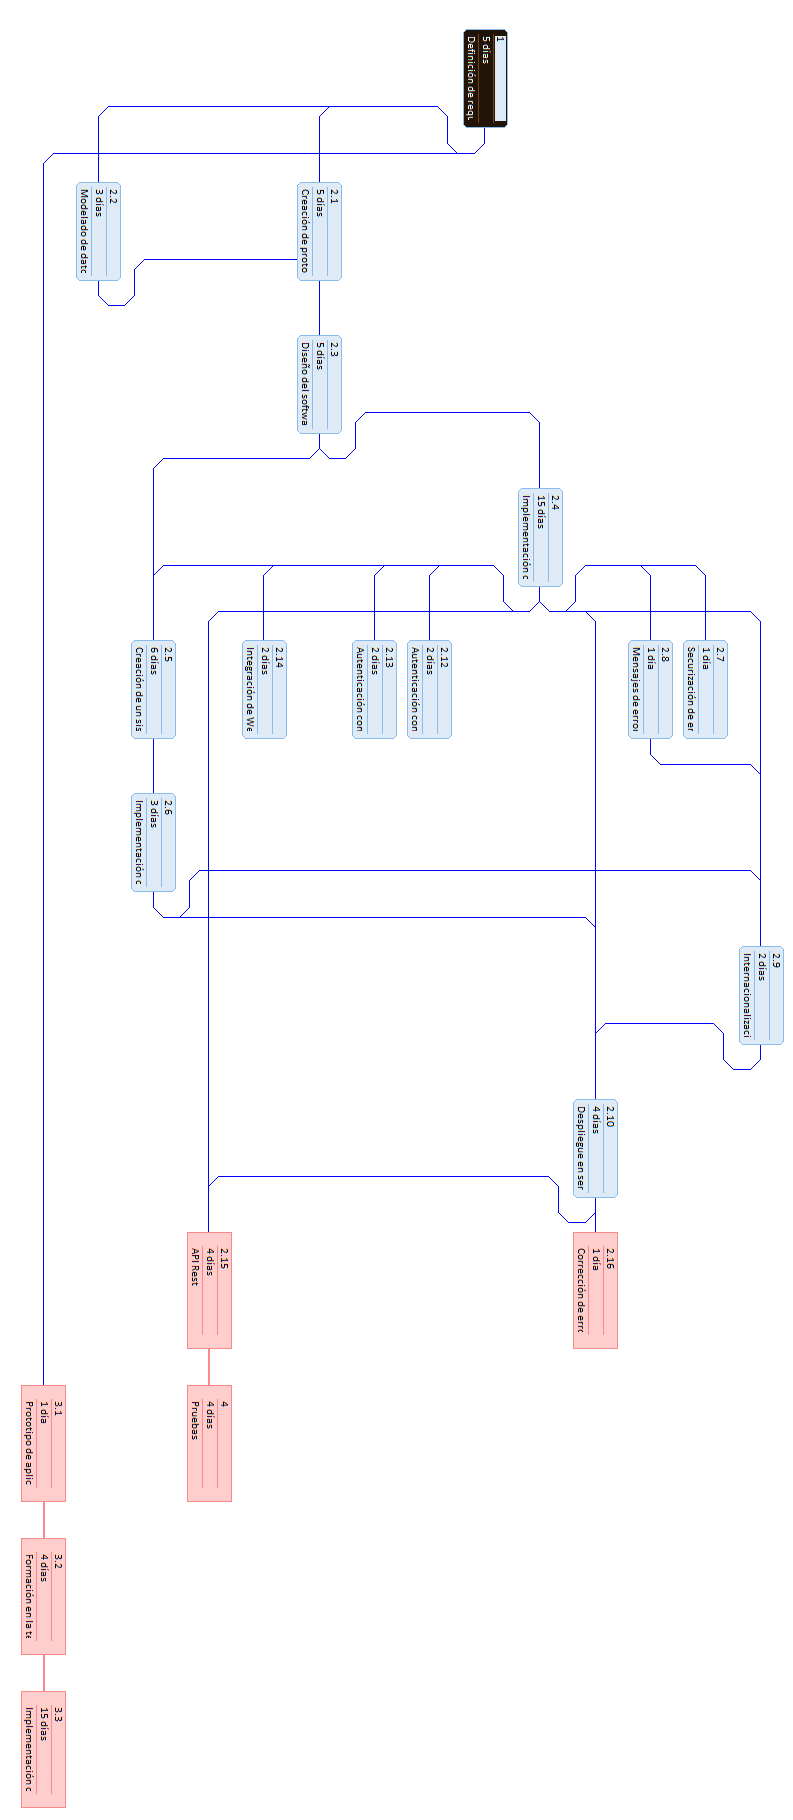
\includegraphics[width=210pt]{fig/precedencia}
	\caption{Precedence diagram}\label{fig:precedencediagram}
\end{figure}

\backmatter

\end{document}
